%  LaTeX support: latex@mdpi.com 
%  For support, please attach all files needed for compiling as well as the log file, and specify your operating system, LaTeX version, and LaTeX editor.

%=================================================================
\documentclass[life,article,submit,pdftex,moreauthors]{Definitions/mdpi} 

%% The amssymb package provides various useful mathematical symbols
\usepackage{amssymb}
%% The amsmath package provides various useful equation environments.
\usepackage{amsmath}
%% The amsthm package provides extended theorem environments
%% \usepackage{amsthm}
\usepackage{array}
\usepackage{tabularx}
\usepackage{booktabs}
\usepackage{algorithm}
\usepackage{algorithmic}

%=================================================================
% MDPI internal commands - do not modify
\firstpage{1} 
\makeatletter 
\setcounter{page}{\@firstpage} 
\makeatother
\pubvolume{1}
\issuenum{1}
\articlenumber{0}
\pubyear{2025}
\copyrightyear{2025}
%\externaleditor{Academic Editor: Firstname Lastname}
\datereceived{ } 
\daterevised{ } % Comment out if no revised date
\dateaccepted{ } 
\datepublished{ } 
%\datecorrected{} % For corrected papers: "Corrected: XXX" date in the original paper.
%\dateretracted{} % For corrected papers: "Retracted: XXX" date in the original paper.
\hreflink{https://doi.org/} % If needed use \linebreak
%\doinum{}
%\pdfoutput=1 % Uncommented for upload to arXiv.org
%\CorrStatement{yes}  % For updates

%=================================================================
% Full title of the paper (Capitalized)
\Title{Stability-Driven Assembly as a Natural Genetic Algorithm}


% MDPI internal command: Title for citation in the left column
\TitleCitation{Stability-Driven Assembly as a Natural Genetic Algorithm}

% Author Orchid ID: enter ID or remove command
\newcommand{\orcidauthorA}{0009-0007-7122-0317} % Add \orcidA{} behind the author's name

% Authors, for the paper (add full first names)
\Author{Dan Adler $^{1}$\orcidA{}}

% MDPI internal command: Authors, for metadata in PDF
\AuthorNames{Dan Adler}

% Affiliations / Addresses
\address{%
$^{1}$ \quad dan@danadler.com}

%=================================================================
% Abstract (Do not insert blank lines, i.e. \\) 
\abstract{
This paper presents Stability-Driven Assembly (SDA), a framework in which selection emerges from persistence imbalances rather than externally specified fitness. In SDA, assemblies are created stochastically and persist according to stability. Longer-lived motifs become overrepresented and more likely to participate in future interactions, yielding fitness-proportional sampling and thus a natural genetic algorithm (SDA/GA). We instantiate SDA in chemical symbol space using fragment recombination and single-site mutations with a heuristic stability function. Simulations produce oligopolistic population structures, convergence of scaffold families, heavy-tailed rank–abundance distributions, and characteristic entropy/diversity dynamics consistent with selection. We contrast these findings with equilibrium analyses (e.g., constant-rate models), which suppress selection-driven evolution. We propose that SDA/GA is not only a model of chemical dynamics but a universal systemic process: in any universe where stochastic assembly, replenishment, and differential persistence coexist, populations are inevitably skewed and selection-like dynamics emerge. This reframes the central dogma that evolution requires replication, suggesting instead that replication is one rung in a broader ladder that begins with persistence, catalysis, and autocatalysis. SDA/GA thus provides a unifying principle linking chemistry, computation, and biology, and suggests that the emergence of information-rich order may be an inherent outcome of physical law.
}


% Keywords
\keyword{Stability-Driven Assembly; Natural Genetic Algorithms; Emergent dynamics; Information dynamics; Origins of life; Persistence-driven selection; Evolutionary pathways}

%=================================================================
\begin{document}

\section{Introduction}

One of the deepest questions in the origins of life research is how selection could operate before the advent of replication. Biological evolution depends on variation and inheritance, but both presuppose molecular mechanisms capable of copying information. However, long before such machinery existed, physical and chemical systems already exhibited differences in persistence: some structures survived longer than others under given conditions. The central question is whether these persistence imbalances, acting alone, are sufficient to generate selection-like dynamics and drive the emergence of complexity.

In inanimate systems, patterns persist according to their stability under prevailing conditions. Diamonds outlast graphite under high pressure, and certain molecular motifs are more resilient in given chemical environments \cite{ruizmirazo2014}. Here we use motif to mean a distinct pattern—or, in chemical contexts, a distinct species. Such differences in longevity create implicit selection: stable structures naturally accumulate, biasing the population distribution. This principle of stability-driven selection may provide a bridge between non-living matter and evolving biospheres \cite{kauffman1993origins, hordijk2012autocatalytic, nghe2015prebiotic}.

Multiple theoretical frameworks have addressed how complexity might emerge from abiotic systems. Autocatalytic-set theory shows how reaction networks can become self-sustaining \cite{kauffman1986autocatalytic, hordijk2011required}. Eigen's hypercycles \cite{eigen} extend this idea to mutually reinforcing replicators, but still presuppose replication machinery. Fontana's artificial chemistry \cite{fontana1991algorithmic} and later digital artificial life platforms such as \textit{Tierra} and \textit{Avida} \cite{ray1992tierra, adami1994} demonstrated open-ended dynamics in abstract symbolic systems. More recently, Cronin’s chemputation approach has automated chemical synthesis \cite{cronin2024chemputation}, showing how chemistry can be controlled as code, although only under the guidance of an external programmer. The GARD model of lipid assemblies \cite{segre2000compositional, markovitch2012universal} and protocell ABMs \cite{damer2015coupled} demonstrate how compositional inheritance can arise in specific chemistries. Each of these frameworks contributes valuable insight, yet they remain tied to particular substrates or assume replication.

Other perspectives highlight general physical drivers: preferential attachment in networks \cite{barabasi1999emergence}, dissipative adaptation in nonequilibrium thermodynamics \cite{prigogine1977self, england2015dissipative}, and work on evolutionary dynamics in chemical networks \cite{wu2012origin, nowak2006evolutionary}. Assembly Theory quantifies complexity as construction depth \cite{walker2023nature}, while constructor theory reformulates physics in terms of possible transformations \cite{deutsch2013constructor}. These approaches offer tools to measure or formalize complexity, though they stop short of explaining how information-generating dynamics arise in real time.

The phrase 'chemical evolution' is widely used in the literature to describe the progressive transformation of molecules into more complex structures under prebiotic conditions. Yet the term is often applied descriptively rather than mechanistically, leaving open the question of what underlying principle imparts directionality or selection to such processes. In particular, while many models demonstrate how complexity can arise in specific chemistries, a general account of how chemical systems move from undirected reaction networks to cumulative, evolutionary dynamics has remained elusive.

This paper introduces Stability-Driven Assembly (SDA) as a framework in which 
selection arises from persistence imbalances alone. Each generation is shaped 
by two processes: stochastic creation of new assemblies and persistence or 
decay according to stability. Together, these processes form a feedback cycle
in which stable motifs accumulate and bias future sampling, effectively implementing roulette-wheel selection in the sense of a genetic algorithm (GA) 
\cite{holland1975adaptation, adler1993marriage}, but without an externally
imposed fitness function.

Applied to organic chemistry, SDA simulations with chemically meaningful
recombinations and mutations show populations progressively dominated by
increasingly stable compounds, driving the system toward order while
occasional stochastic innovations trigger bursts of reorganization.

\section{Stability-Driven Assembly (SDA)}

A Stability-Driven Assembly (SDA) \cite{adler_sda} system consists of base elements $A, B, C, \dots$ that recursively combine into compounds represented as
strings of unbounded length. The persistence of each compound is determined by its
stability $S$: a compound with $S=30$ remains for 30 generations before elimination, while the patterns $S=1$ vanish after a single generation. 
Expired motifs are removed without explicit reverse reactions and base
elements are replenished at a constant rate each generation, ensuring
continued exploration of assembly space. This setup parallels continuous-flow 
stirred tank reactors (CFSTR) \cite{fogler1999chemical}, where reactants are
continuously supplied to maintain non-equilibrium conditions. More formally, An SDA system is defined as a tuple $(E, P, S, R, I)$ where:
\begin{itemize}
   \item $E = \{e_1, e_2, \ldots, e_n\}$ is a finite set of base elements
   \item $P$ is the set of all possible patterns formed by concatenating elements from $E$ and existing patterns
   \item $S: P \rightarrow \mathbb{Z}^{+}$ is a stability function mapping each pattern to a positive integer representing its lifetime
   \item $R: E \rightarrow \mathbb{Z}^{+}$ is a replenishment function specifying how many copies of each base element are added per generation
   \item $I \in \mathbb{Z}^{+}$ is the number of interactions allowed per generation
\end{itemize}
The pattern interaction operation, denoted by $\oplus$, is defined as a string concatenation. When patterns $p_1$ and $p_2$ interact, they form a pattern $p_1 \oplus p_2$.

\begin{algorithm}[H]
\caption{SDA System Simulation}
\begin{algorithmic}[1]
\REQUIRE Base elements $E$, stability $S$, replenish $R$, interactions $I$, generations $T$
\ENSURE Pattern population evolution over $T$ generations
\STATE Initialize population with base elements
\FOR{$t = 1$ to $T$}
   \STATE Remove expired patterns
   \STATE Add $R(e)$ copies of each element $e \in E$ to population
   \FOR{$i = 1$ to $I$}
       \STATE Select patterns $p_1$, $p_2$ randomly from population
       \STATE Form $p_{new} = p_1 \oplus p_2$
       \STATE Set expiration time for $p_{new}$ to $t + S(p_{new})$
       \STATE Add $p_{new}$ to population
   \ENDFOR
\ENDFOR
\end{algorithmic}
\end{algorithm}


The probability of selecting a pattern $p$ for interaction is proportional to its frequency in the population. This creates a feedback mechanism: patterns with higher stability persist longer, becoming more abundant, which increases their probability of participating in interactions.

The original SDA formulation emphasizes string concatenation as the sole
pattern-forming operation. In what follows, we generalize the interaction 
to a recombination operator with an optional mutation step, and then examine 
whether the core properties of SDA are preserved under this extension. 
We refer to this generalized version as \textit{SDA/GA}, since the dynamics 
are formally equivalent to those of a genetic algorithm while retaining 
persistence as the implicit fitness measure. Instead of:
\[
p_{\text{new}} = p_1 \oplus p_2
\]
we use a recombination of the two patterns:
\[
p_{\text{new}} = \mathrm{Recombine}(p_1, p_2)
\]
optionally followed by \emph{single–site mutation} applied with probability $\mu$:
\[
p_{\text{new}} =
\begin{cases}
\mathrm{Mutate}(p_{\text{new}}) & \text{with probability } \mu,\\
p_{\text{new}} & \text{with probability } 1-\mu
\end{cases}
\]
This change does not alter the selection mechanism: persistence $S(p)$ still 
determines residence time and thus induces roulette–wheel selection.


\subsection{Population and Stability Distributions}

SDA dynamics are captured by two complementary distributions. 
The \textit{population distribution} tracks the relative abundance of each pattern:
\begin{equation}
P_t(p) = \frac{N_t(p)}{\sum_{q \in P} N_t(q)},
\end{equation}
where $N_t(p)$ is the count of the pattern $p$ in generation $t$. 
The \textit{stability function}, $S: P \rightarrow \mathbb{Z}^+$, assigns each pattern a characteristic lifetime. 
In chemical implementations, these lifetimes could in principle be derived from binding energies, activation barriers, or other domain-specific stability measures.

\subsection{Pattern Evolution Model}

In \cite{adler_sda} we derived a simple persistence–creation update rule where 
recombination was modeled as deterministic concatenation. This took the form
\begin{equation}
\label{eq:create-term-simple}
\mathrm{Create}_t(p) = \sum_{(q,r)\to p} P_t(q)\,P_t(r),
\end{equation}
where $(q,r)\to p$ denotes parent pairs that yield $p$ by concatenation. 
Together with the persistence term
\begin{equation}
\label{eq:persist-term-simple}
\mathrm{Persist}_t(p) = P_t(p)\left(1-\frac{1}{\overline{R}_t(p)}\right),
\end{equation}
where $\overline{R}_t(p)$ denotes the mean remaining lifetime of all active
instances of $p$ at time $t$. This gives a baseline recursive update. To handle recombination more generally, we now allow a parent pair $(q,r)$ 
to produce not just one deterministic child but a distribution of possible
offspring. We capture this by introducing a recombination-mutation kernel
$K_t(p\mid q,r)$, which gives the probability that $q$ and $r$ produce
offspring $p$ at time $t$:
\begin{equation}
\label{eq:create-term-kernel}
\mathrm{Create}_t(p) = \sum_{q,r\in P} P_t(q)\,P_t(r)\,K_t(p\mid q,r),
\qquad \sum_{p\in P} K_t(p\mid q,r)=1~\forall~q,r.
\end{equation}
The persistence term remains as in Eq.~\ref{eq:persist-term-simple}. Intuitively, $K_t$ is just a lookup table of possible children for each 
parent pair. In the deterministic concatenation case, it reduces to 
$K_t(p\mid q,r)=\mathbf{1}\{p=q\oplus r\}$, so each pair produces exactly 
one child. In recombination, $K_t$ may spread probability mass across 
several outcomes: most weight might go to $q\oplus r$, but smaller weight 
can go to shorter or mutated variants. This makes explicit how mutation 
and recombination introduce variation, while preserving the same update 
structure as before. The updated population distribution is then
\begin{equation}
\label{eq:full-ba-update}
P_{t+1}(p) = \frac{\mathrm{Persist}_t(p) + \mathrm{Create}_t(p)}
{\sum_{p' \in P} \big[\mathrm{Persist}_t(p') + \mathrm{Create}_t(p')\big]}.
\end{equation}

Thus, the kernel-based formulation extends the earlier model in a minimal
way: concatenation is a special case, and recombination with mutation is
just a richer offspring distribution. This does not alter the persistence-driven drift, which remains governed entirely by stability. The kernel instead modifies the structure of the creation term, enriching the range of variants without changing the underlying bias toward stability.


\subsection{Entropy Dynamics}

The Shannon entropy of the population at time $t$ is defined as
\begin{equation}
H(P_t) = - \sum_{p \in P} P_t(p) \log_2 P_t(p).
\end{equation}
Changes in entropy reflect the balance between novelty introduced by creation and order enforced by persistence.
\begin{equation}
\Delta H = H(P_{t+1}) - H(P_t).
\end{equation}
To quantify this balance, we define
\begin{equation}
\alpha = \frac{\sum_p \mathrm{Persist}_t(p)}
{\sum_p \mathrm{Persist}_t(p) + \sum_p \mathrm{Create}_t(p)}.
\end{equation}
When $\alpha \to 1$, stability dominates and entropy tends to decrease; when $\alpha \to 0$, creation dominates and entropy tends to increase.  
A first-order approximation expresses the entropy change as a weighted combination of these contributions:
\begin{equation}
\Delta H \approx (1 - \alpha)\,\Delta H_{\text{create}} + \alpha\,\Delta H_{\text{persist}},
\end{equation}
where $\Delta H_{\text{create}}$ is typically positive and $\Delta H_{\text{persist}}$ negative.  The interaction of these opposing forces explains the oscillatory entropy trajectories sometimes observed in simulation, as phases of innovation alternate with phases of stabilization.

\subsection{Continuum Limit and Fokker-Planck Analogy}

In the continuum limit, the SDA update can be written in a Fokker-Planck form \cite{gardiner2009}:
\begin{equation}
\frac{\partial P(x,t)}{\partial t}
= \underbrace{- \nabla \cdot \big[ A[P](x,t)\, P(x,t) \big]}_{\text{Persist / drift}}
+ \underbrace{D \nabla^2 P(x,t)}_{\text{Create / diffusion}}.
\end{equation}
Here $P(x,t)$ is the probability density of observing motif $x$ at time $t$, 
serving as the continuous analogue of the discrete distribution $P_t(p)$. 
The drift term $A[P](x,t)$ is not fixed externally but depends functionally on $P$: 
it reflects the evolving stability landscape shaped by the current population. 

Thus, although the equation resembles a linear Fokker-Planck, it is in fact nonlinear and path-dependent. 
The first-order operator ($\nabla$) represents persistence-driven drift toward regions of higher stability, 
while the second-order operator ($\nabla^2$) captures diffusion-like spreading from stochastic creation. 
This functional dependence makes SDA dynamics intrinsically nonequilibrium and distinguishes them from 
classical Fokker-Planck systems where drift and diffusion are externally specified. 
Formally, SDA belongs to the class of nonlinear Fokker-Planck systems sometimes called McKean--Vlasov equations \cite{mckean1966, villani2009}, 
where drift depends self-consistently on the evolving distribution.  

As demonstrated in our previous intervention experiments \cite{adler_sda}, 
\textit{Persist} (stability imbalances) is the intrinsic driver of entropy
reduction and pattern persistence, whereas \textit{Create} serves as a uniform ergodic source of novelty that cannot itself generate order.  
In the continuum formulation, these two contributions map onto drift and diffusion, 
but unlike the classical case, the drift field is a functional of the evolving
population itself.  

This makes the SDA equation fundamentally different from the classical Fokker-Planck equation of equilibrium statistical mechanics. In standard treatments, 
drift and diffusion are externally specified, yielding linear operators that
permit eigenfunction expansions and closed-form steady states. In contrast,
in SDA the drift emerges endogenously from the evolving distribution $P(x,t)$, 
rendering the process non-linear, feedback driven and intrinsically non-equilibrium.  
As a result, traditional solution techniques based on linear operators and
stationary distributions are not directly applicable, highlighting the need
for alternative approaches in the SDA framework.


\subsection{Symbolic Simulation Model Parameters}

All symbolic SDA and Unconstrained simulations below used a common set of parameters. The base elements are $A$, $B$, $C$.
Each generation included
a replenishment of 5 base elements and 100 random pairwise
interactions. In the unconstrained simulations, all the resulting patterns had the same stability of 1 generation. For the SDA simulations, 
stability values were assigned to patterns according to the
function:

\begin{equation}
S(p) =
\begin{cases}
100, & \text{if } p = \text{ABCABA} \\
50, & \text{if } p \in \{\text{ABA, ABC}\} \\
30, & \text{if } p \in \{\text{AB, BC}\} \\
1, & \text{otherwise}.
\end{cases}
\end{equation}

These parameters were fixed in the symbolic experiments below, ensuring that the observed differences arose from the interventions rather than changes in
the baseline setup.

\begin{figure}[H]
    \centering
    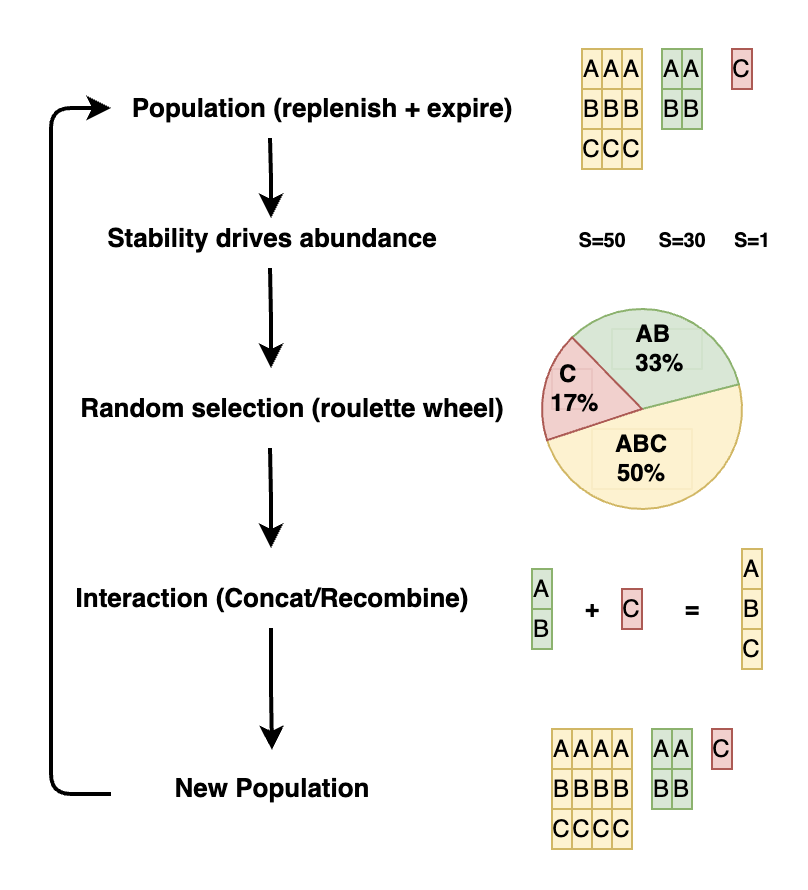
\includegraphics[width=0.75\textwidth]{SDA-Sym.png}
    \caption{Symbolic SDA/GA loop in ABC space. 
    Base elements are replenished and unstable motifs expire, forming the current population. 
    Stability values ($S=50,30,1$) skew motif abundance, producing a biased distribution (pie chart). 
    Random selection operates by roulette-wheel sampling proportional to this abundance. 
    Selected motifs undergo interaction (concatenation in SDA, recombination in GA), 
    generating new assemblies that enter the next population. 
    This feedback cycle: stability $\to$ persistence $\to$ population skew $\to$ biased sampling yields emergent fitness-proportional selection without an explicit fitness function.}
    \label{fig:sda-loop}
\end{figure}

Figure~\ref{fig:sda-loop} illustrates how these parameters operate within the
symbolic SDA/GA loop. Replenishment and expiration define the active population, 
stability values skew motif abundance, and roulette-wheel sampling drives
biased parent selection. Interactions (concatenation or recombination) then
produce new motifs that re-enter the pool, closing the feedback cycle. 
This diagram highlights how persistence alone induces effective selection
pressure without an explicit fitness function.

\subsection{Simulation Results}

We begin by comparing the final pattern distributions produced by the original SDA with concatenation and the generalized SDA/GA with recombination. Both systems show a strong deviation from the unconstrained case: instead of a uniform spread of short strings, high-stability motifs dominate the population. In the SDA system, concatenation drives the emergence of long-repeated motifs such as \texttt{ABCABA}, which accumulate a lot of the probability mass. In the recombination-based GA variant, the same dominant motifs appear, but the distribution shows a heavier tail: many low-frequency variants persist alongside the stable core (Figures~\ref{fig:concat-patterns},~\ref{fig:ga-patterns}). This broader spectrum reflects the ability of recombination to continuously inject mosaic offspring and maintain a pool of rare types, while pure concatenation channels more strongly into layered repeats.

\begin{figure}[H]
    \centering
    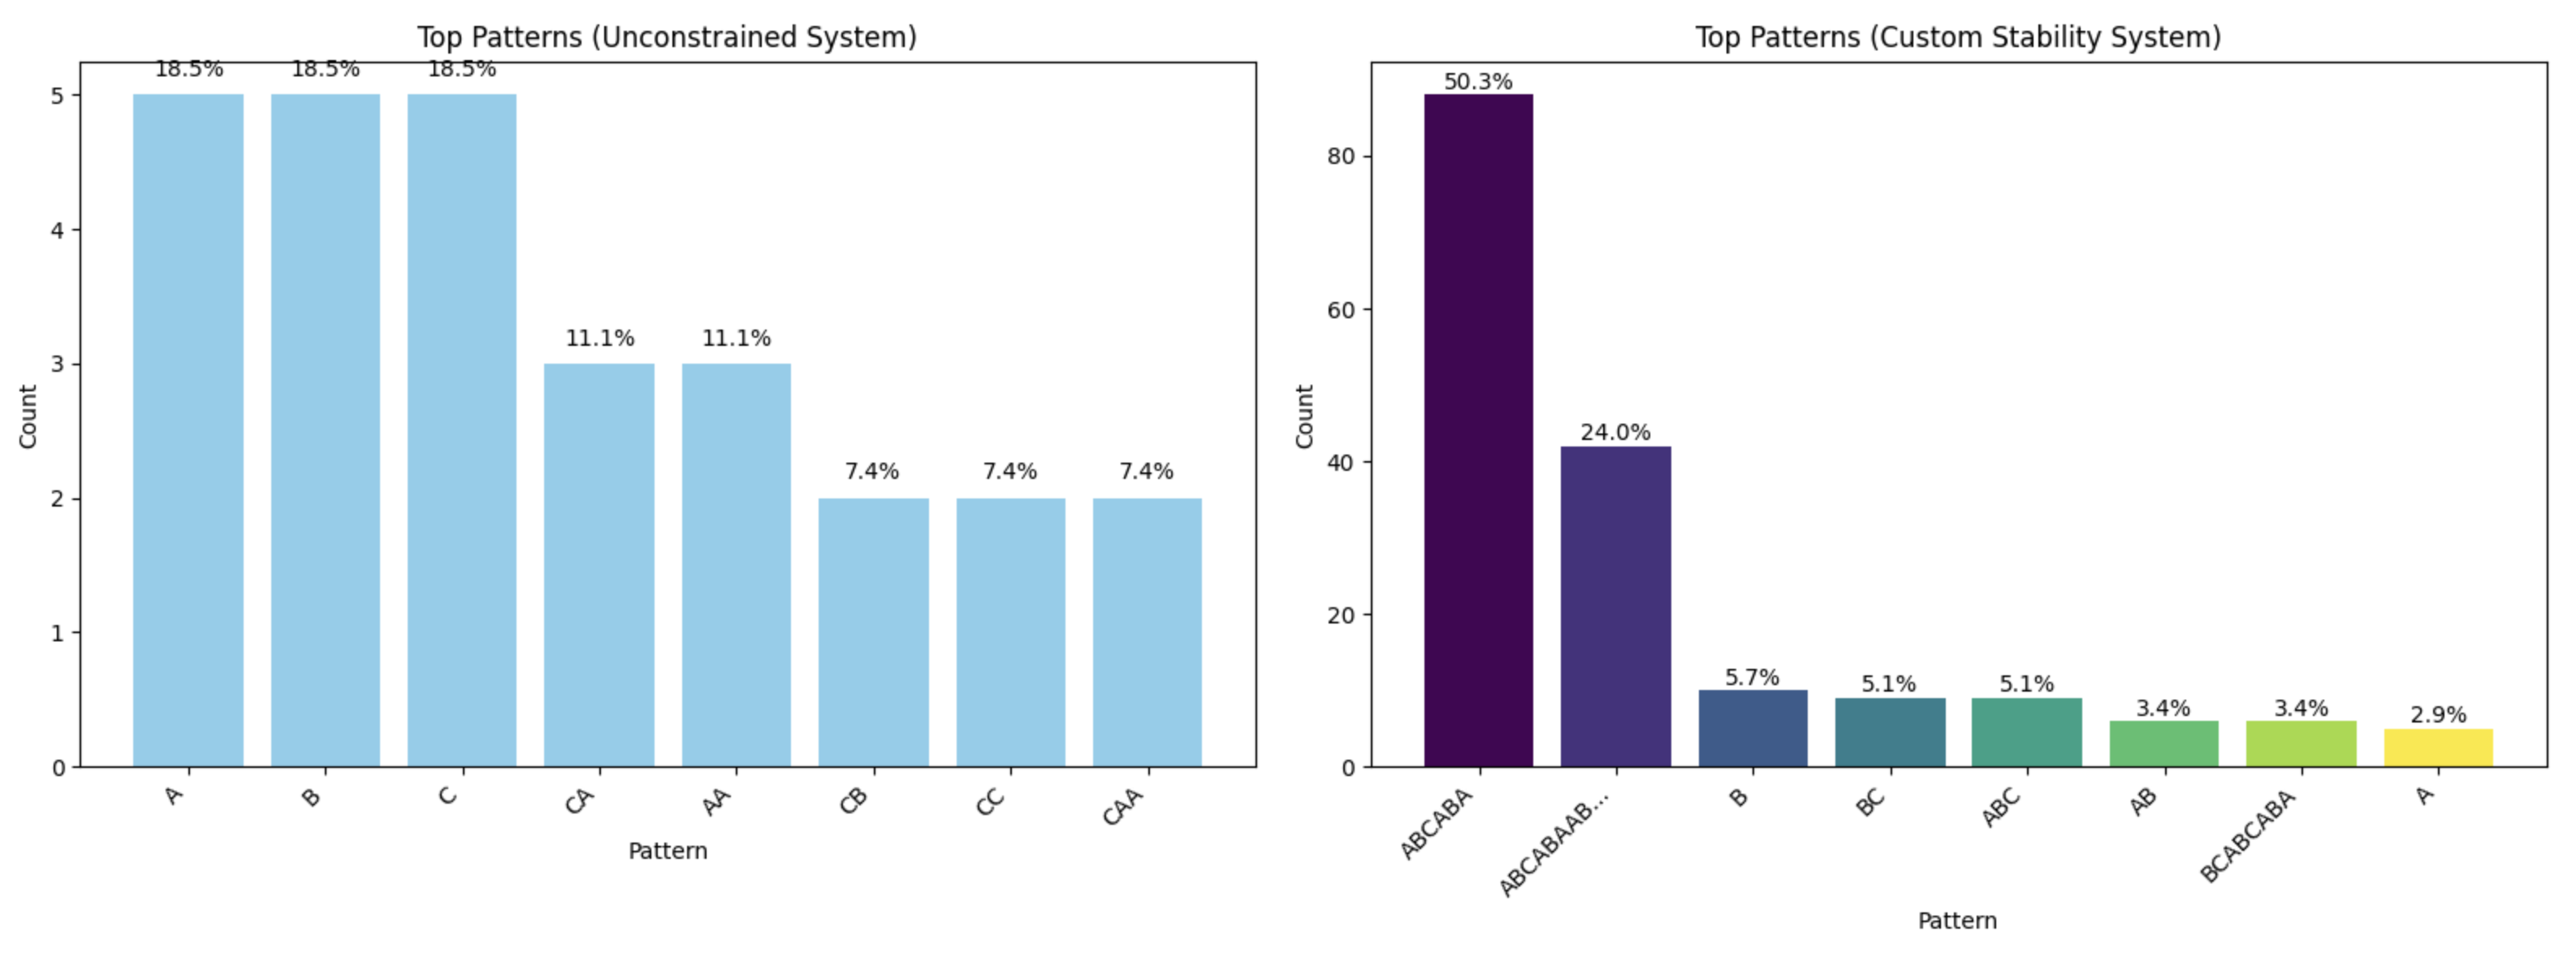
\includegraphics[width=1\textwidth]{SDA-concat-patterns.png}
    \caption{Pattern distribution in the SDA system with concatenation. A small set of high-stability motifs dominate the population, while other patterns are nearly absent.}
    \label{fig:concat-patterns}
\end{figure}

\begin{figure}[H]
    \centering
    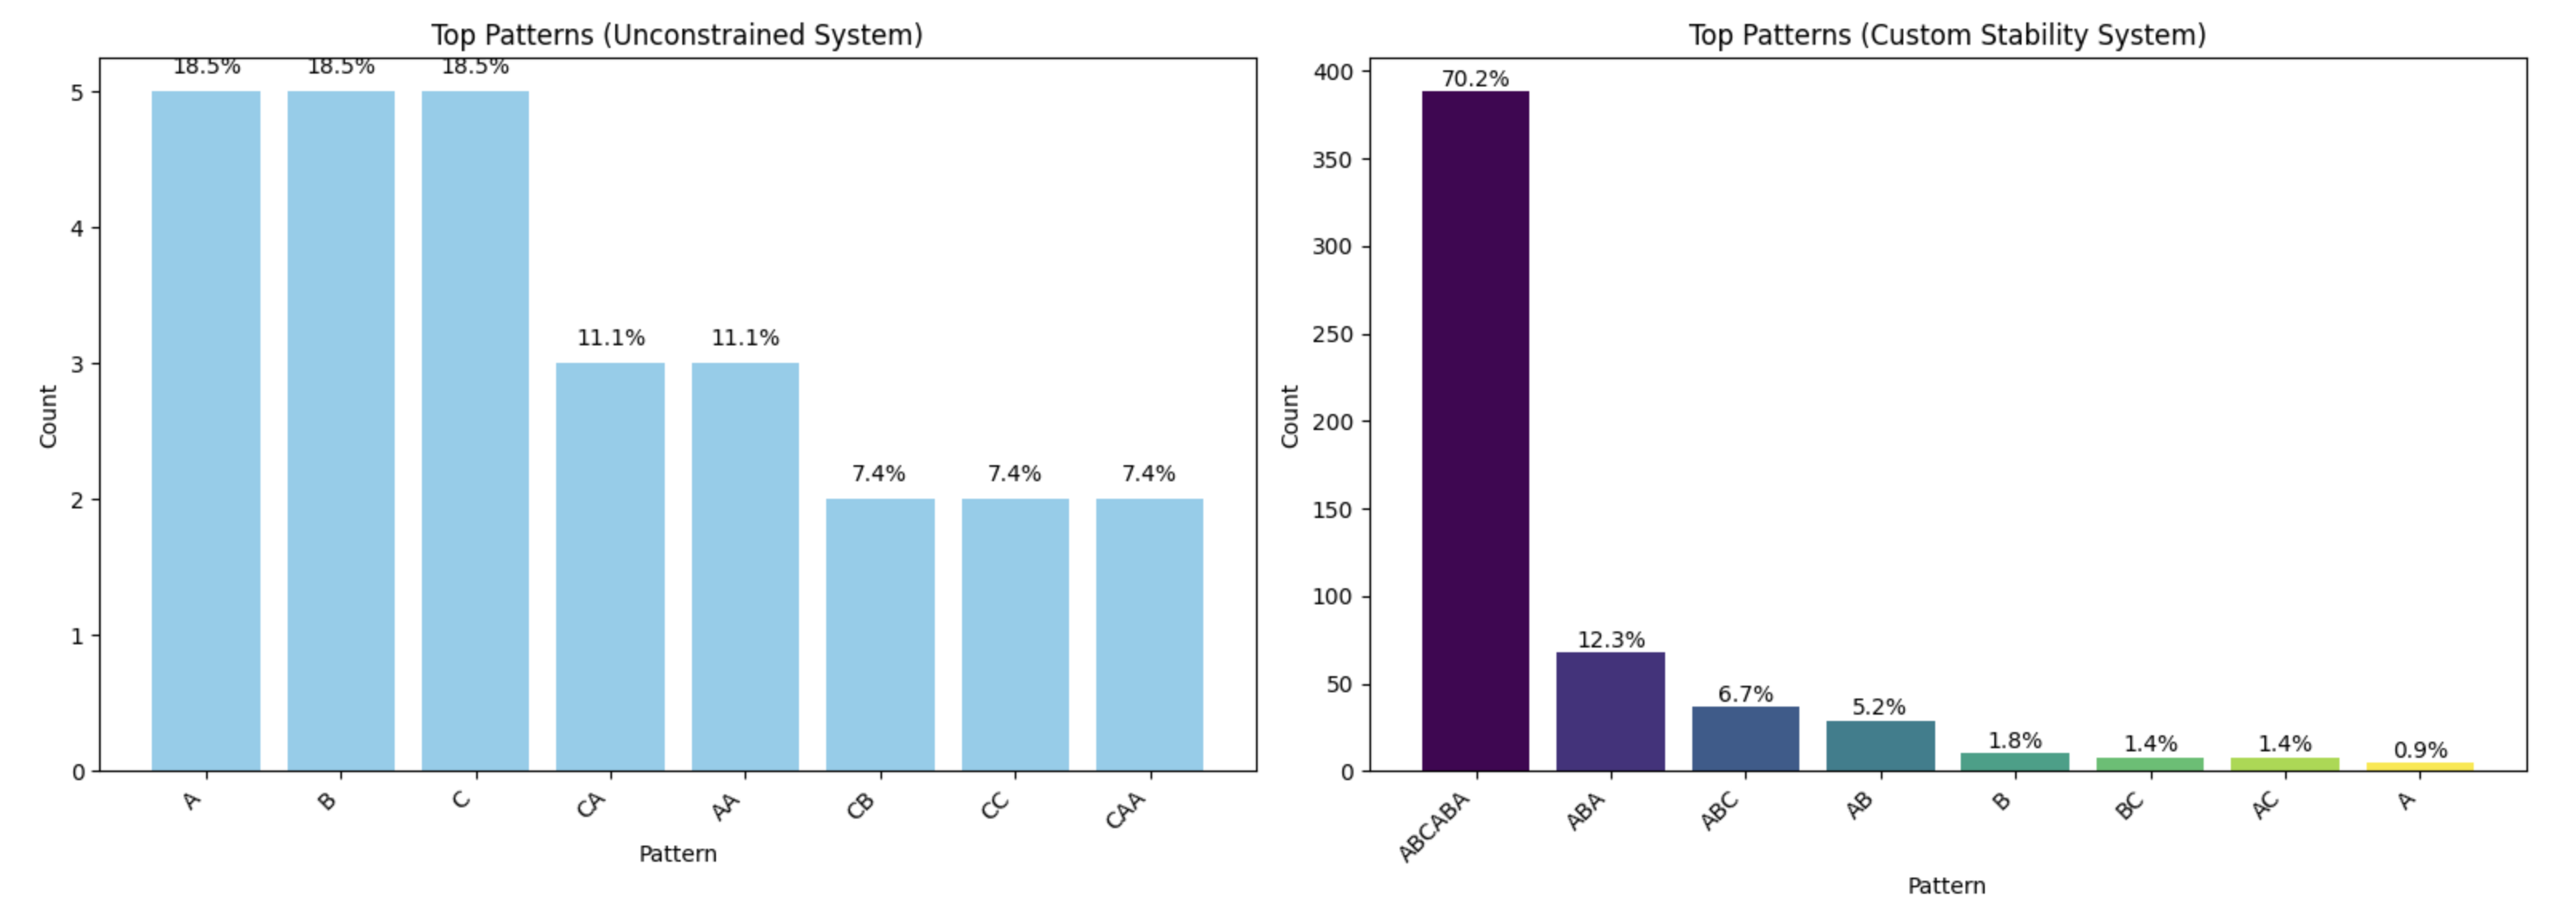
\includegraphics[width=1\textwidth]{SDA-GA-patterns.png}
    \caption{Pattern distribution in the generalized SDA/GA system with recombination. Stable motifs dominate as in the pure SDA case, but a broader tail of low-frequency variants persists due to recombination.}
    \label{fig:ga-patterns}
\end{figure}

In terms of entropy dynamics, both systems show a clear reduction in Shannon entropy ($H(P_t) = - \sum_{p \in P} P_t(p) \log_2 P_t(p)$) of
the pattern distribution in generation t measured in bits relative to the unconstrained baseline, confirming the emergence of order and the presence of selection pressure (Figures~\ref{fig:concat-entropy},~\ref{fig:ga-entropy}). Importantly, this occurs without any explicit fitness-proportional selection rule in the algorithm: roulette-wheel selection emerges intrinsically from persistence, since patterns with longer lifetimes are overrepresented and thus more likely to be sampled for further interactions.

In the concatenation-based SDA, while the average entropy decreases from $\sim6$ bits to $\sim4$ bits, its trajectories often exhibit oscillations. These arise because concatenation tends to build large, synchronized cohorts of similar long motifs that expire at nearly the same time. When such a cohort collapses, replenished base elements briefly increase diversity and entropy before new dominant motifs emerge, creating a characteristic boom–bust cycle. In contrast, in the SDA/GA based on recombination, the entropy decreases more smoothly to $\sim3$ bits without oscillations. Recombination produces mosaic offspring with staggered lifetimes, desynchronizing expirations, and damping collective turnover. The result is a more monotonic entropy collapse toward a skewed distribution anchored by stable motifs.

\begin{figure}[H]
\centering
\subfloat[\centering Concatenation-based SDA]{
    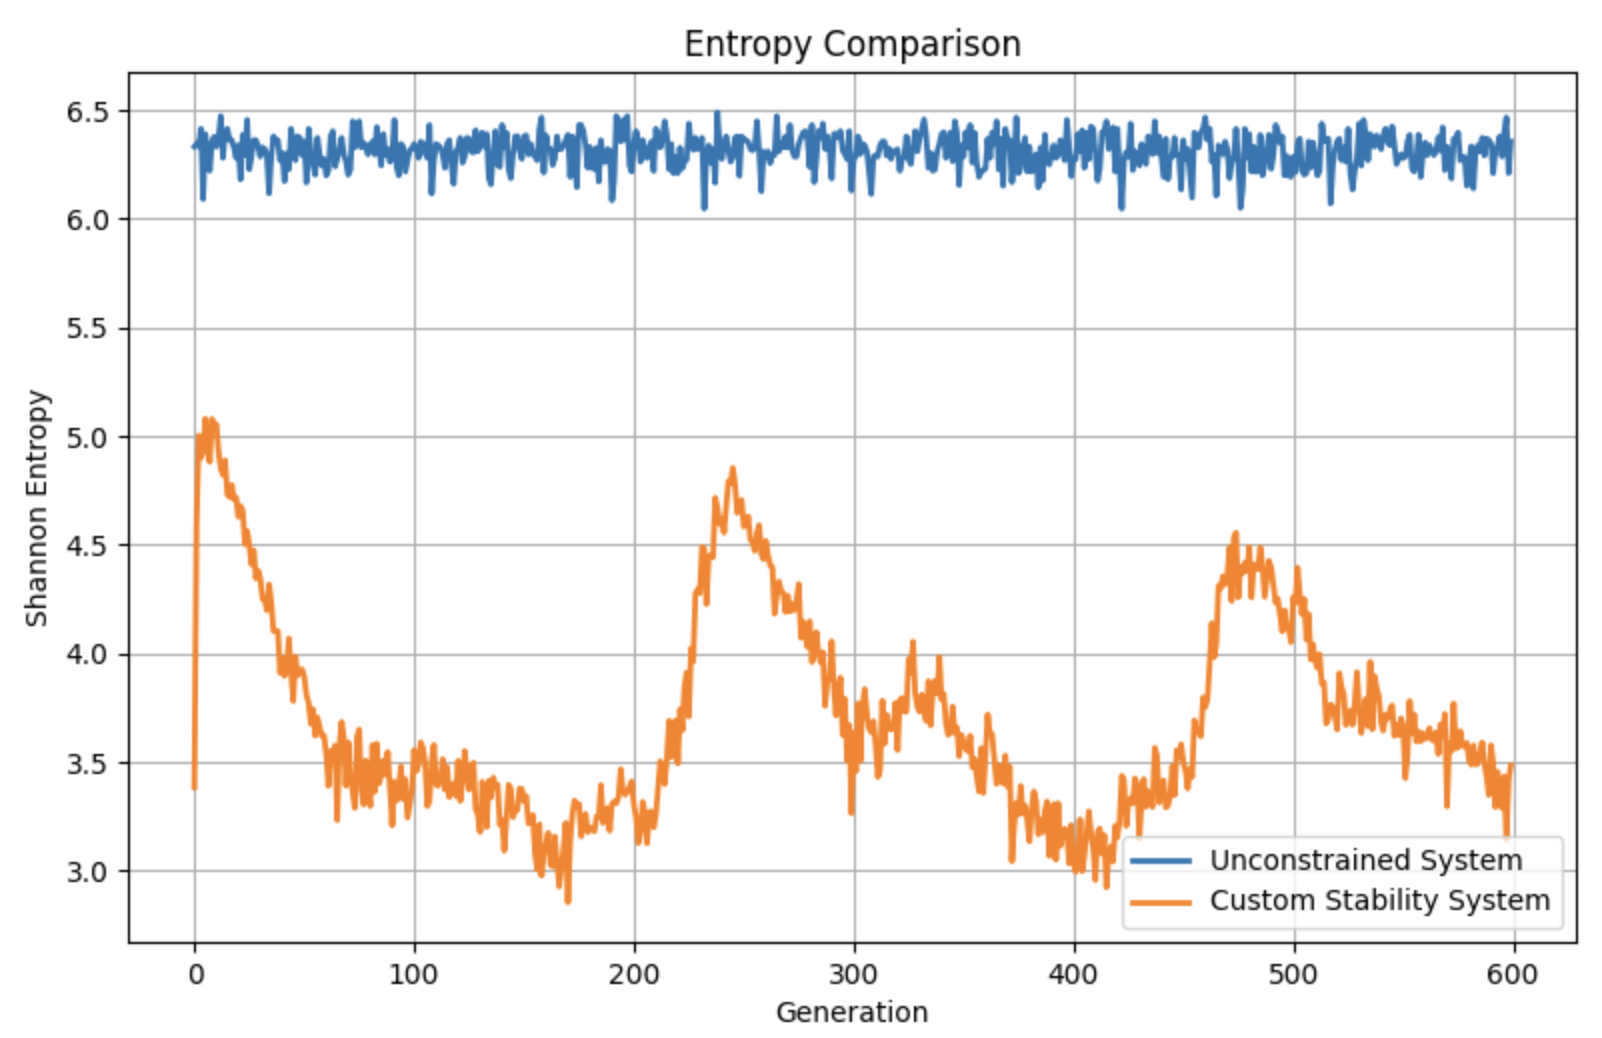
\includegraphics[width=0.45\textwidth]{SDA-concat-entropy.png}
    \label{fig:concat-entropy}
}
\hfill
\subfloat[\centering Recombination-based SDA/GA]{
    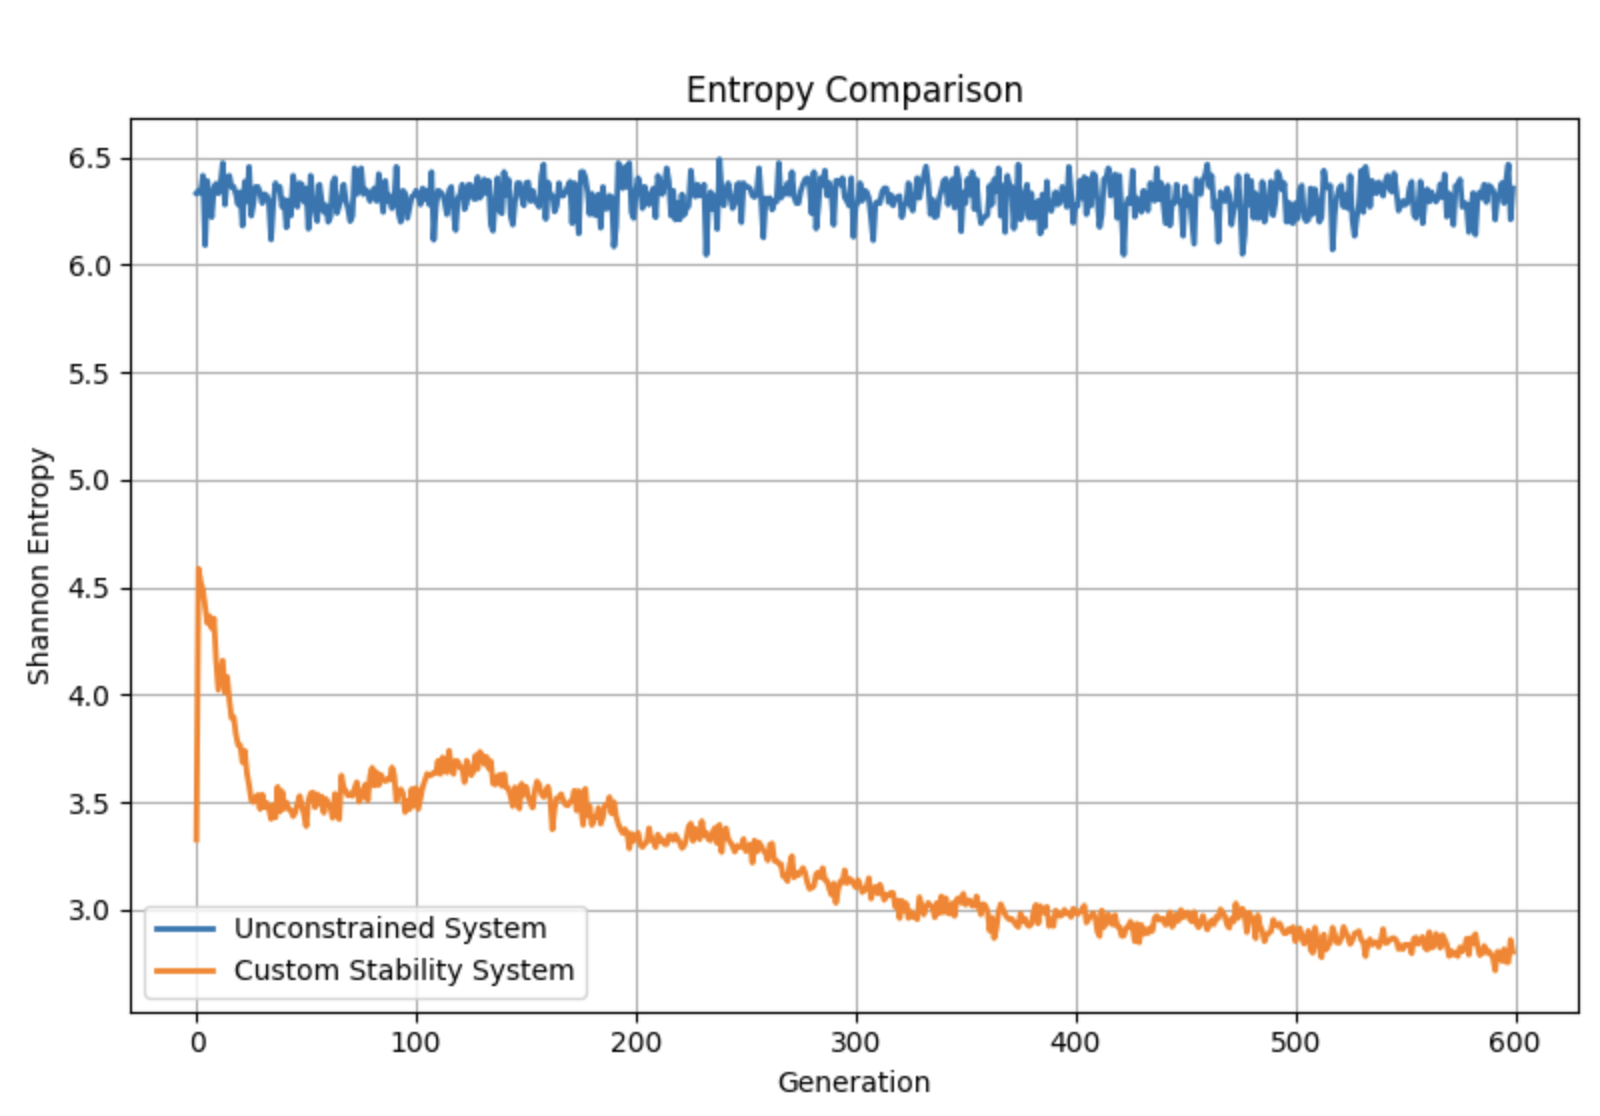
\includegraphics[width=0.45\textwidth]{SDA-GA-entropy.png}
    \label{fig:ga-entropy}
}
\caption{Entropy dynamics under different operators. (\textbf{a}) Concatenation-based SDA shows oscillatory boom–bust cycles due to synchronized expiration of long motifs. (\textbf{b}) Recombination-based SDA/GA shows smoother entropy decline, as recombination desynchronizes expirations.}
\label{fig:entropy-comparison}
\end{figure}


Together, these results demonstrate that stability-driven assembly robustly yields emergent selection pressure and entropy reduction under both concatenation and recombination operators. The choice of interaction operator primarily shapes the dynamical form of convergence: oscillatory cycles under concatenation versus smooth decline under recombination.

\begin{figure}[H]
\centering
\subfloat[\centering Concatenation-based SDA]{
    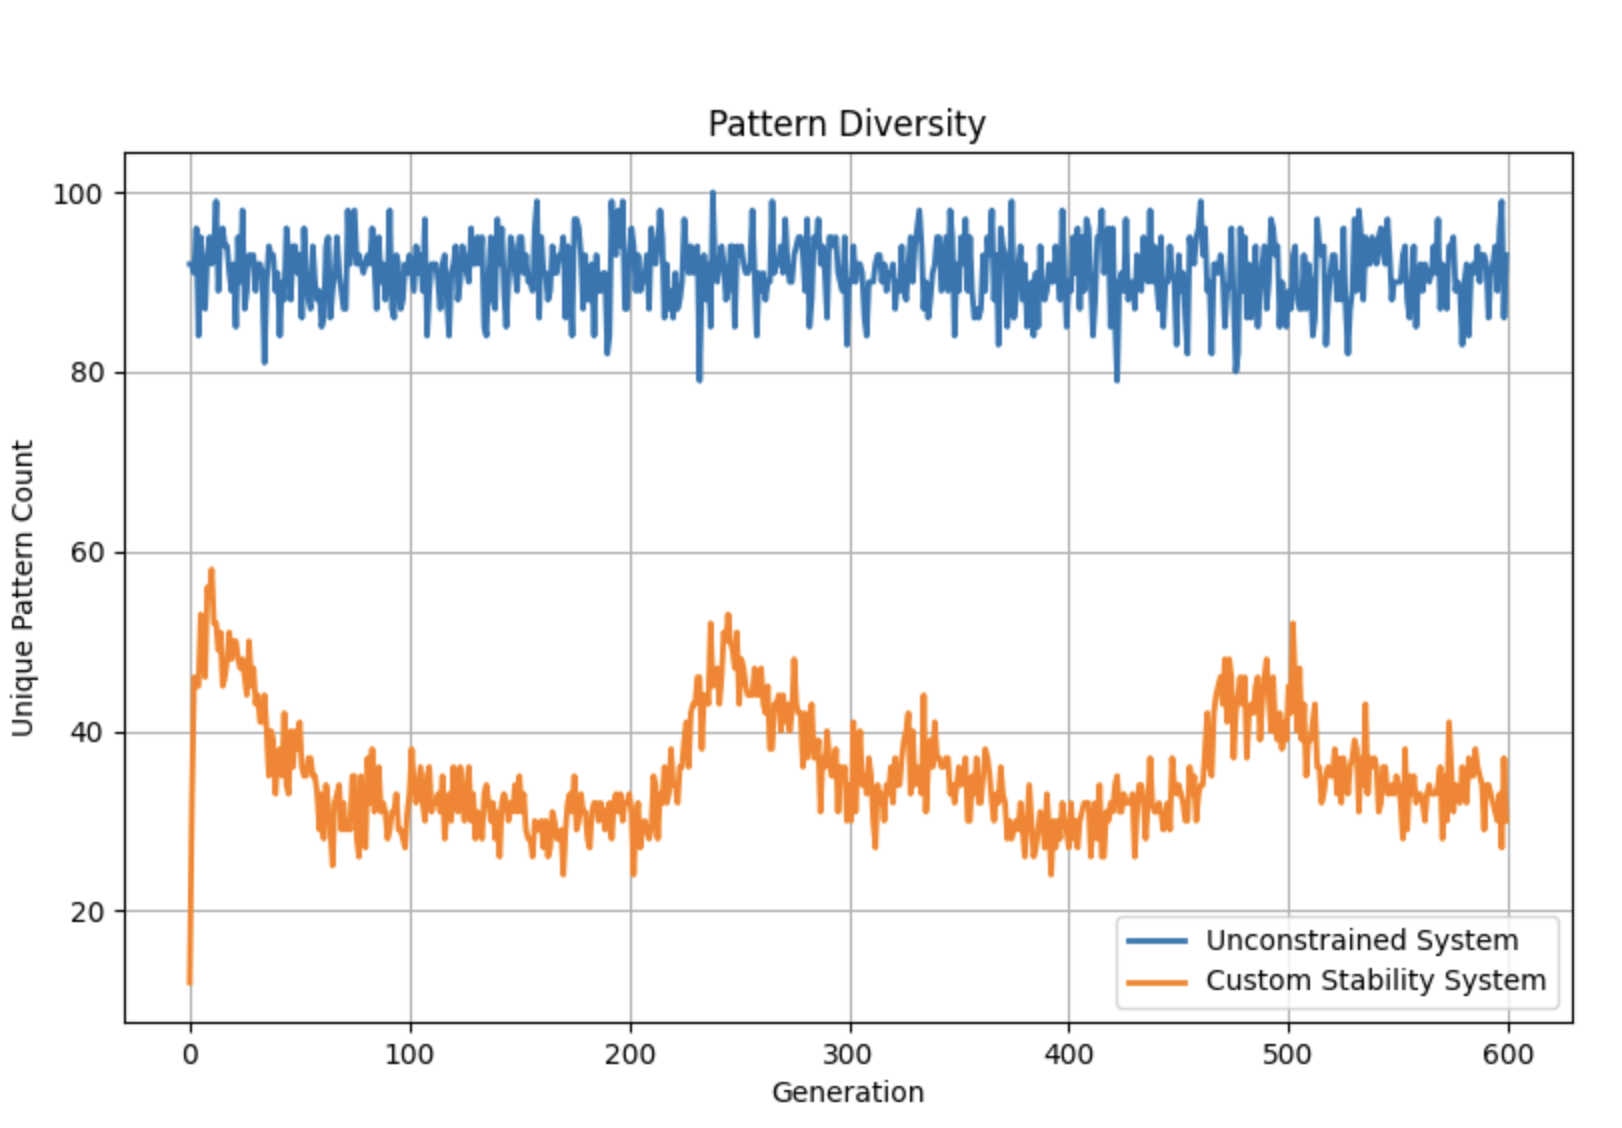
\includegraphics[width=0.45\textwidth]{SDA-concat-diversity.png}
    \label{fig:concat-diversity}
}
\hfill
\subfloat[\centering Recombination-based SDA/GA]{
    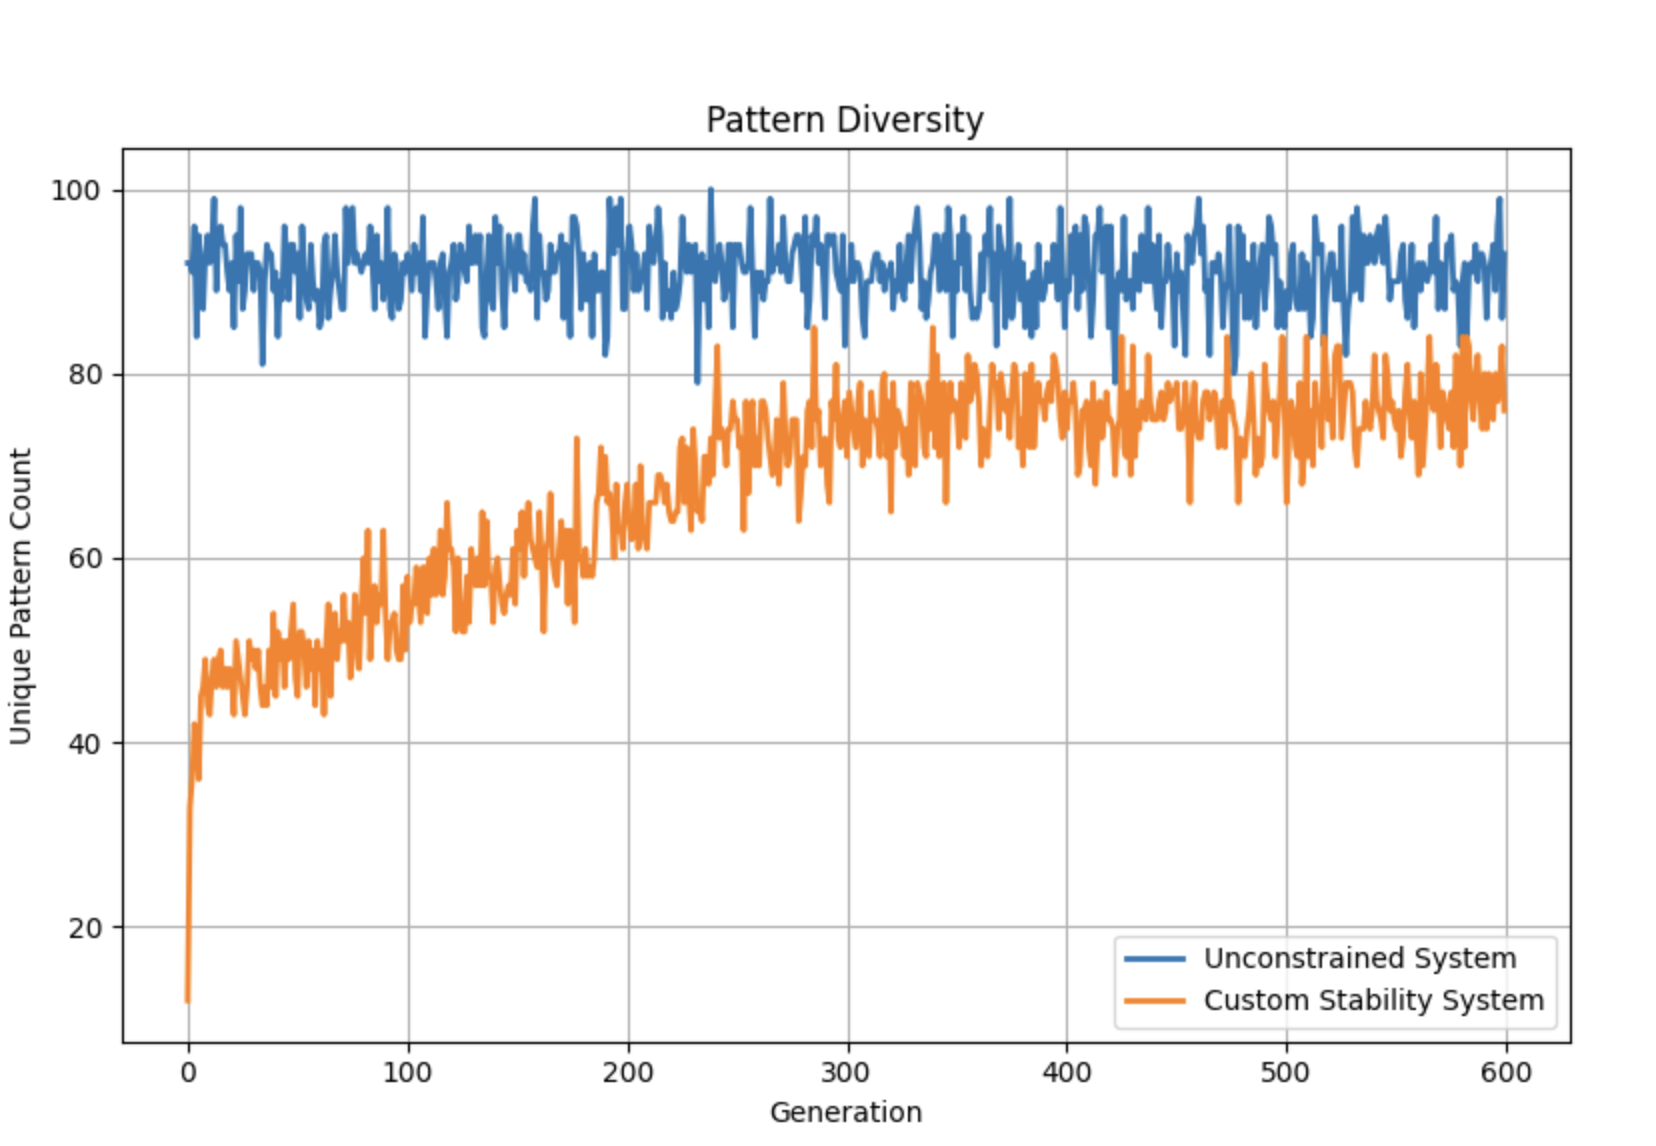
\includegraphics[width=0.45\textwidth]{SDA-GA-diversity.png}
    \label{fig:ga-diversity}
}
\caption{Pattern diversity under different operators. (\textbf{a}) Concatenation-based SDA shows oscillations, reflecting synchronized motif turnover and boom--bust dynamics. (\textbf{b}) Recombination-based SDA/GA shows steadily rising diversity, indicating continuous generation of low-frequency variants.}
\label{fig:diversity-comparison}
\end{figure}


The unique pattern diversity results in Figures~\ref{fig:concat-diversity} and~\ref{fig:ga-diversity} highlight the exploration--exploitation tradeoff. 
In concatenation-based SDA, exploration of pattern space is intermittent: 
diversity rises when base elements re-enter, then collapses as a dominant 
motif takes over, producing oscillatory boom--bust dynamics. In contrast, 
recombination-based SDA/GA sustains a broader exploration of the space, 
with diversity approaching unconstrained levels even though entropy 
collapses. Most of these additional patterns remain low-probability, but 
their presence shows that recombination and mutation inject continuous 
novelty. Thus, SDA/GA combines strong exploitation of stable motifs with 
ongoing exploration of alternatives---a hallmark of genetic algorithms---all 
emerging naturally without an explicit fitness function.


We also tested the effect of introducing low-probability single-site mutations during recombination. 
These mutations serve as a simple model of stochastic perturbations such as copying errors or
diffusion events. As expected, mutation did not qualitatively alter the dynamics: entropy
collapsed and high-stability motifs remained dominant. Mutations did not disrupt the overall reduction in entropy, confirming that the emergent selection mechanism is robust to stochastic noise.

\section{Genetic Algorithms and Natural Genetic Algorithms}

The study of genetic algorithms (GAs) has a long history in computer science and optimization. 
Holland’s foundational work \cite{holland1975adaptation} introduced the idea of using crossover, 
mutation, and selection to evolve solutions to computational problems. Later, Goldberg 
\cite{goldberg1989genetic} popularized and formalized GAs as practical optimization tools, 
particularly for engineering and combinatorial search. Building on this tradition, Koza 
\cite{koza1992genetic} extended the paradigm to genetic programming (GP), in which whole 
program trees rather than fixed-length strings evolve under crossover and mutation. GP has 
been especially influential in symbolic regression and in evolving nontrivial structures such 
as circuits, strategies, and controllers.

In all of these approaches, the defining feature of a GA or GP is that the \emph{fitness function} 
is externally specified by the programmer. The GA loop evaluates each candidate solution, assigns 
a fitness value, and uses that fitness to bias the sampling of parents. Whether the goal is 
minimizing error in a regression task or maximizing throughput in a design problem, the selective 
pressure is supplied by the problem designer.


In contrast, in a Stability-Driven Assembly (SDA) system, the selection mechanism is not externally
programmed but emerges intrinsically from persistence. Each pattern has a stability $S(p)$, 
which determines how long it remains in the population. Patterns with higher stability survive
longer, become more frequent, and are therefore more likely to be sampled for further
recombination. This effectively implements a roulette-wheel selection scheme without explicitly specifying one in the algorithm.

In simple string models, the stability function $S$ can be assigned by hand to highlight specific motifs, making the dynamics easy to visualize. However, in real-world contexts, the stability
function is determined by the environment itself. In chemistry, for example, molecular stability 
arises from thermodynamics, kinetics, and reaction constraints. In biology, environmental conditions 
determine whether a sequence or structure persists. Thus, while a traditional GA requires the 
programmer to provide an explicit fitness function, a natural GA---as instantiated by SDA---derives 
its fitness measure from the environment. This distinction is crucial for interpreting SDA not just as an algorithmic metaphor but as a model of how nature itself performs search and selection.

Classical GA uses an explicit programmer-supplied fitness function $f$ to bias selection. 
In SDA, there is no explicit selection operator: Each pattern $p$ receives a stability
$S(p)$ that sets its expiration time $t_{\exp}(p)=t+S(p)$. Patterns with larger $S(p)$ 
persist longer and are therefore sampled more often for recombination, resulting in fitness proportional selection without computing $f$. 
For toy strings, $S$ may be assigned by design; for realistic chemistry, $S$ is determined 
by the environment (valence/duet–octet satisfaction, sterics, thermodynamics, kinetics, 
reactor residence time). Thus, SDA \emph{builds fitness into persistence}, while GA
\emph{supplies fitness explicitly}.

One well-known illustration of genetic algorithms is the Dawkins 'weasel' program \cite{dawkins1986blind}, where random sequences evolve
toward a fixed target phrase through repeated variation and selection. 
It shows how cumulative selection outperforms random search, but only
because an externally defined goal and fitness function are imposed. 
This target-driven design contrasts with the open-ended dynamics modeled
here.  

An analogy closer to SDA is jazz improvisation \cite{adler2025jazz}. 
Musicians explore an open-ended space of motifs within a predefined harmonic space
without a fixed target. Motifs that resonate are repeated, varied, and recombined, while others fade. Musical structure thus emerges from this stochastic but biased search. 
Similarly, SDA explores assembly space, persistence bias amplifies
stable motifs, and novelty accumulates without a prespecified goal. 
Both processes discover order by letting persistence guide variation, 
illustrating how information can emerge from feedback rather than
external targets.


\section{Application to Organic Chemistry}

The abstract SDA/GA framework can be instantiated in the chemical symbol space to model
the spontaneous evolution of molecular populations. In this setting, the base elements
$E$ are drawn from the atomic alphabet (C, O, N, H, etc.), and the interaction operator
$\oplus$ is instantiated as recombination and mutation of molecular fragments. 

Genetic algorithms and genetic programming have long been applied in chemistry and 
cheminformatics, particularly for de novo molecular design and drug discovery 
\cite{brown2004ga,lewis1998gp,jensen2019ga,yoshikawa2018ga}. These approaches typically 
represent molecules as graphs or strings and apply crossover and mutation operators 
guided by an externally defined fitness function, such as binding affinity, 
drug-likeness, or synthetic accessibility. Fink and Reymond’s construction of the
GDB-11 database \cite{fink2007gdb11} demonstrated the sheer size of chemically valid
search space, generating over 26 million molecules with up to 11 atoms and over
110 million stereoisomers. However, only a small fraction of these compounds occur in
public databases, underscoring both the vastness of chemical possibility and the impracticality of a uniform or ergodic search. This observation motivates the use of
search strategies that inherently bias exploration toward persistent and chemically
stable motifs. Whereas traditional GA/GP methods rely on explicit, human-specified 
fitness functions to impose such bias, the SDA/GA framework does so intrinsically by
embedding stability into persistence, allowing selection pressure to emerge directly
from environmental constraints such as valence rules, steric feasibility, and
thermodynamics.

It is important to emphasize that the present work is not aimed at drug discovery
or molecular optimization applications, which have been the traditional focus of
genetic algorithms and genetic programming in chemistry. Instead, our goal is
conceptual: to hypothesize how nature itself may have acted as a 'natural genetic algorithm', using stability-driven persistence as the implicit fitness function to
non-ergodically explore the astronomical chemical space revealed by studies such
as GDB-11. Within this perspective, the emergence of a biosphere can be viewed as
the outcome of stability-biased sampling: persistent motifs accumulate, dominate, 
and recombine, gradually transforming an unconstrained chemical universe into a
structured, evolving system.


The mapping in Table~\ref{tab:chem-sda-operators} illustrates how common classes of organic reactions can be interpreted within the SDA/GA framework. Substitution, reduction and oxidation reactions all correspond to \textit{mutations}, since they alter functional groups while preserving the underlying scaffold. Addition reactions may play either role: the attachment of a small atom or group is best regarded as mutation, whereas the joining of two larger fragments constitutes recombination.  

Acid-base reactions are a particularly simple but important form of mutation. Protonation and deprotonation cycles alter charge states and stability without changing the covalent backbone, yet they have profound effects on persistence in different environments. Similarly, isomerization represents a mutational step in which the connectivity or geometry is reshuffled, sometimes uncovering stability differences that bias persistence even though no atoms are gained or lost.  

Polymerization, including peptide bond formation, provides a canonical example of recombination. Here, motifs are linked through edge-biased joining to form larger assemblies. Once formed, such chains introduce new levels of persistence and complexity, laying the groundwork for the higher rungs of the evolutionary ladder. Fragmentation and dissociation serve as the inverse of recombination, redistributing persistence across smaller motifs.  

This mapping shows that the SDA operators of mutation and recombination are not abstract inventions but correspond directly to well-established categories of chemical reactivity. This correspondence grounds the abstraction in chemical reality and illustrates how stability-driven selection could operate in real chemical networks without requiring additional operators beyond those already available to organic chemistry.


\begin{table}[H]
\caption{Representative mappings between classical organic reactions and SDA operators.\label{tab:chem-sda-operators}}
\begin{adjustwidth}{-\extralength}{0cm}
\begin{tabularx}{\fulllength}{XXX}
\toprule
\textbf{Reaction Type} & \textbf{Representative Example} & \textbf{SDA Analogy} \\
\midrule
Substitution / Redox & R--CHO $\leftrightarrow$ R--CH$_2$OH / R--COOH & Mutation: functional group replaced or bond order changed. \\
\midrule
Addition & R--C=O + R'X $\to$ R--C(OH)X & Recombination if full fragment joins; mutation if small group adds. \\
\midrule
Acid--Base & R--NH$_2$ + H$^+$ $\leftrightarrow$ R--NH$_3^+$ & Mutation: reversible protonation state. \\
\midrule
Polymerization & Amino acids $\to$ peptide chains & Recombination of motifs at reactive edges. \\
\midrule
Isomerization & Keto--enol tautomerism & Mutation: structural rearrangement without new parts. \\
\midrule
Fragmentation & Ester hydrolysis (R--COOR' $\to$ R--COOH + R'OH) & Inverse of recombination; persistence split across products. \\
\bottomrule
\end{tabularx}
\end{adjustwidth}
\end{table}

In classical chemistry, reaction types are usually taught as synthesis pathways, 
each requiring defined reagents, catalysts, and conditions. The SDA framework, on the other hand, abstracts these transformations into population-level operators. 
Rather than focusing on the mechanistic sequence of steps, SDA emphasizes how
persistence and recombination biases determine which motifs accumulate over time. 
In this way, SDA complements the traditional synthesis perspective by revealing
how macro-level selection effects emerge from the distribution of possible
transformations.  

Table~\ref{tab:chem-sda-operators} lists representative mappings between
classical reaction classes and SDA operators. To illustrate, 
Figure~\ref{fig:mutation-recombination}a shows a \textit{mutation} event in
which ethanol (CCO) is converted to isopropanol (CC(C)O), a local substitution
that alters stability while preserving the scaffold. 
Figure~\ref{fig:mutation-recombination}b shows a \textit{recombination} event: 
COCCO and CCOC(=O)C combine to yield CCOC, joining fragments from different
parents into a new motif. These cases highlight the two main operator types:
mutations correspond to local functional modifications, while recombinations
generate novelty by linking distinct building blocks.



\begin{figure}[H]
\begin{adjustwidth}{-\extralength}{0cm}
\centering
\subfloat[\centering Mutation]{
  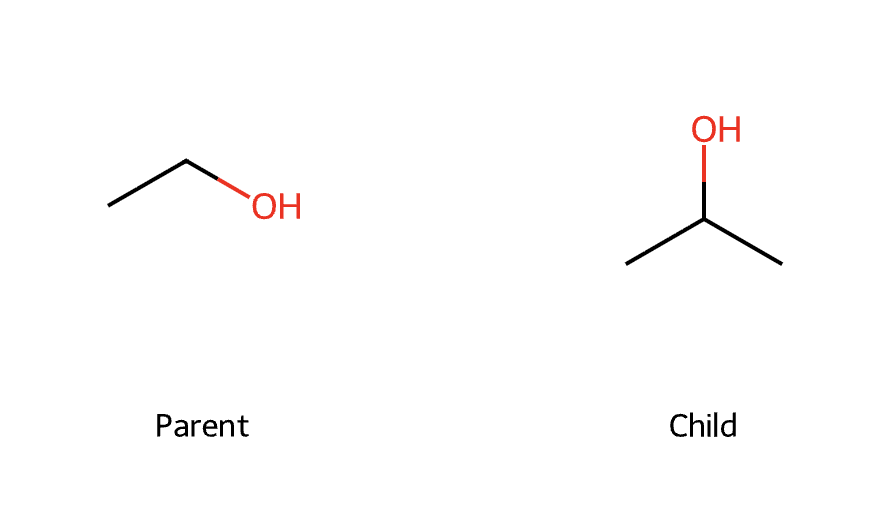
\includegraphics[width=5cm]{mutation_example.png}}
\hspace{0.4cm}
\subfloat[\centering Recombination]{
  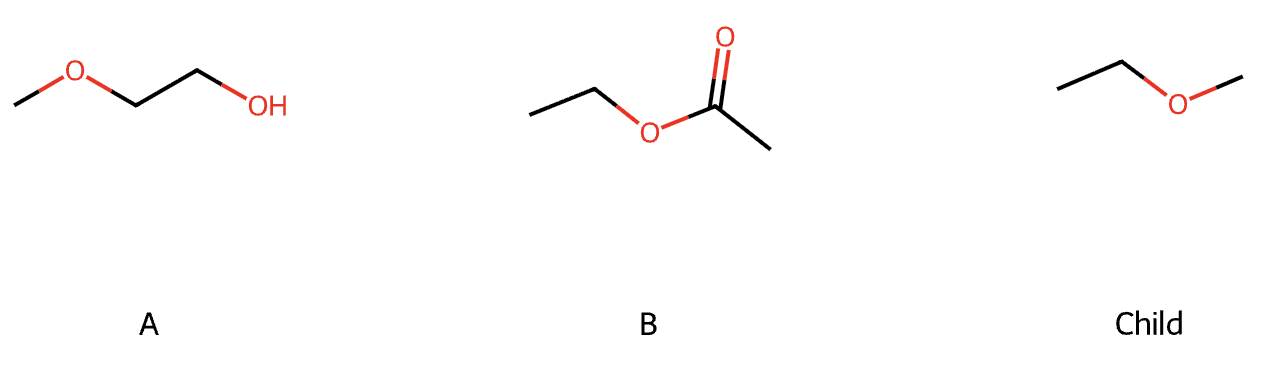
\includegraphics[width=7cm]{recombination_example.png}}
\end{adjustwidth}
\caption{Examples of SDA operators in chemical form. (\textbf{a}) Mutation: ethanol CCO $\to$ isopropanol CC(C)O. 
(\textbf{b}) Recombination: COCCO + CCOC(=O)C $\to$ CCOC.}
\label{fig:mutation-recombination}
\end{figure}

Note that some of these mutations and recombinations do not correspond to single-step reactions in real chemistry and, in practice, may require multistep synthesis pathways, catalysts, or additional energy input. In the SDA framework, however, they are abstracted into single operators in order to isolate the role of persistence bias and population dynamics, leaving mechanistic details to future, more chemically specific implementations.

\begin{figure}[H]
    \centering
    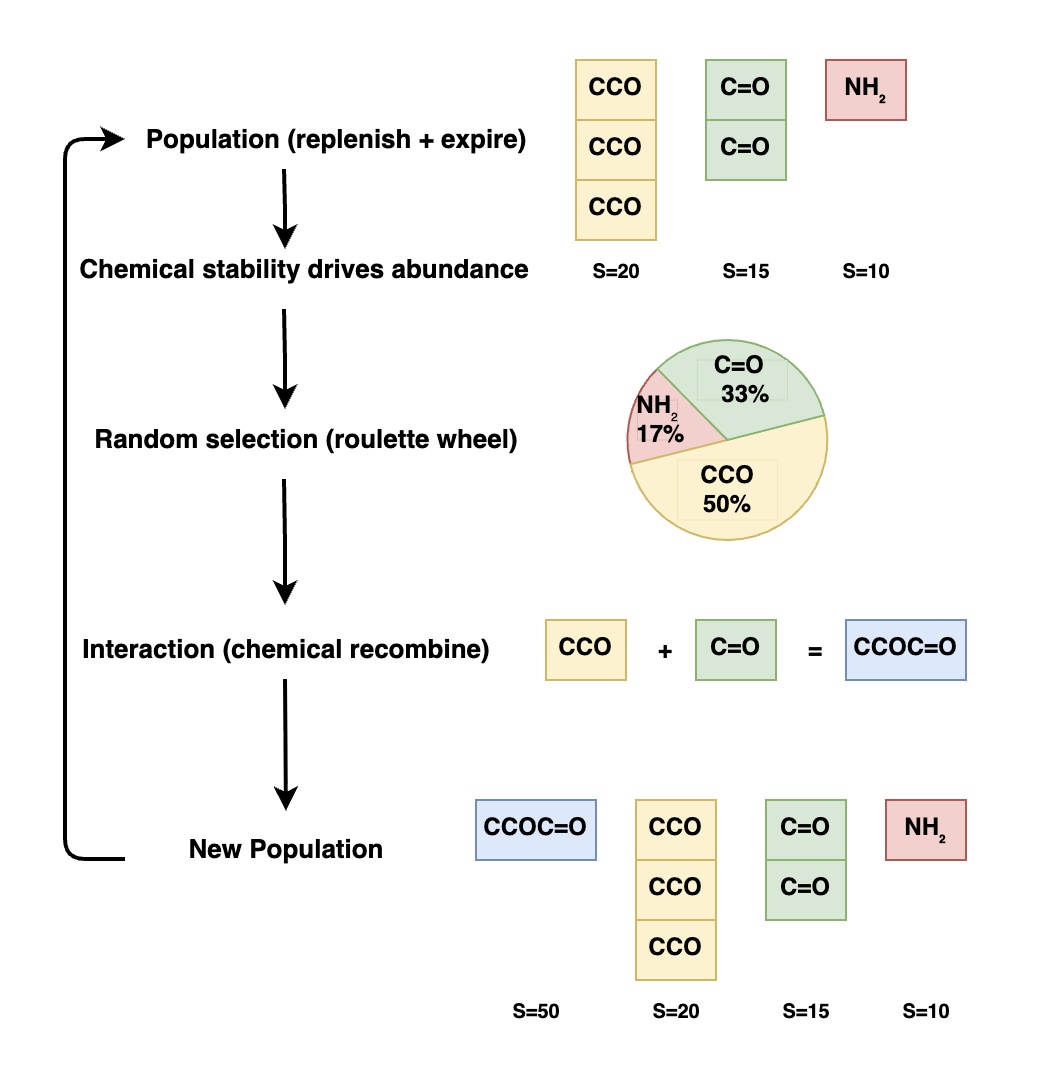
\includegraphics[width=0.75\textwidth]{SDA-Chem.png}
    \caption{Schematic of the SDA/GA loop instantiated in chemical symbol space. 
    The population is replenished and expired each generation, with chemical 
    stability values ($S$) driving the relative abundance of fragments such as 
    ethanol-like \texttt{CCO} ($S=20$), carbonyl \texttt{C=O} ($S=15$), and amine 
    \texttt{NH$_2$} ($S=10$). The resulting abundance distribution biases 
    roulette-wheel selection toward more persistent motifs (here \texttt{CCO} 
    and \texttt{C=O}). Interactions occur through chemical recombination, for 
    example \texttt{CCO + C=O $\to$ CCOC(=O)}, producing more stable compounds 
    ($S=50$) that dominate future populations. The feedback loop illustrates how 
    persistence imbalances alone can generate effective selection dynamics in 
    chemical populations.}
    \label{fig:sda-chem-loop}
\end{figure}

This schematic illustrates the SDA/GA cycle instantiated in the chemical space. As in the symbolic ABC case, persistence bias amplifies the abundance of more stable motifs, which then dominate recombination events and seed increasingly complex products. The point is not to capture mechanistic detail but to show how stability values alone, when coupled with stochastic assembly and replenishment, are sufficient to generate skewed population structures and emergent selection dynamics. In this sense, chemical SDA/GA provides a bridge between abstract population models and realistic prebiotic chemistry.

\subsection{Stability and Environmental Drivers}

In SDA, stability $S(p)$ is defined as persistence between generations: the expected number of time steps that a pattern remains active in the population. This differs from conventional chemical usage, where “stability” usually refers to thermodynamic quantities (e.g., Gibbs free energy) or kinetic barriers (activation energies). Although such energetic factors underlie persistence, SDA abstracts them into a single lifetime parameter that governs how long the motifs continue to participate in the generative process. In this sense, $S(p)$ is not an energy unit, but a phenomenological timescale of survival, informed in practice by thermodynamics, kinetics, and environment.

The environmental drivers are what set these persistence times. Real chemical systems rarely explore assembly space uniformly: reactions depend on conditions such as temperature gradients, pH or redox cycles, porous flows, cofactors, and catalysts, or external inputs such as UV light, electrical discharges, and magnetic fields. Such drivers keep systems away from equilibrium and make persistence differentials consequential. In contrast, laboratory chemistry is usually designed to run to equilibrium, at which point experiments are considered complete, helping explain why reaction networks are seldom framed in evolutionary terms. SDA emphasizes the opposite: In open, driven contexts, replenishment and fluctuation turn heterogeneous persistence into an evolutionary process.  

From this perspective, stability-as-persistence is not an alternative to chemical energetics but a population-level abstraction of their combined effect under environmental drive. Where stochastic assembly, replenishment, and differential persistence coexist, biased sampling and selection-like dynamics naturally emerge.


\section{Chemical SDA/GA Simulation}

\subsection{Methods}
To extend the symbolic SDA/GA framework into the chemical domain, we reused the same minimal simulation loop with two modifications. First, symbolic string elements were replaced with SMILES fragments drawn from a small set of base compounds (e.g., \texttt{C}, \texttt{CC}, \texttt{O}, \texttt{CO}), representing a rudimentary pool of prebiotic building blocks. The molecules were represented as SMILES strings and manipulated using the RDKit toolkit \cite{landrum2006rdkit}. Recombination was implemented through BRICS-based fragmentation and reassembly \cite{degen2008art}, ensuring valence plausibility and avoiding chemically impossible bonds. Mutation was modeled as single-site perturbations, analogous to copying errors or diffusion-induced reactions. These design choices follow established best practices for applying genetic algorithms to molecular discovery \cite{janet2023bestpractices}.

Second, the stability values were no longer fixed but estimated by a callable function $S(p)$ that reflects persistence. In practice, we used simple cheminformatics heuristics (heavy atom count with boosts for motifs such as carboxylates, esters, and amides). More detailed models could incorporate semiempirical energy estimates, kinetic barriers, solvent effects, or experimentally measured lifetimes. In this way, fitness is not externally imposed, but arises from the stability constraints of the environment, consistent with the SDA principle that selection emerges from persistence.

All other aspects of the loop remained unchanged: base fragments were replenished each generation, new compounds were formed by recombination and mutation, and expiration times were determined by $S(p)$. This allows the chemical simulation to be understood as a direct extension of symbolic SDA, with minimal changes distinguishing abstract informational dynamics from physically plausible chemical dynamics.


\subsection{Results}

We ran chemical SDA simulations for 1000 generations with 200 interactions per generation and a replenishment rate of five. The results reveal how stability-driven persistence produces skewed population structures, motif-level evolution, and system-wide dynamics that parallel both genetic algorithms (GAs) and ecological systems.  

\begin{figure}[H]
\begin{adjustwidth}{-\extralength}{0cm}
\centering
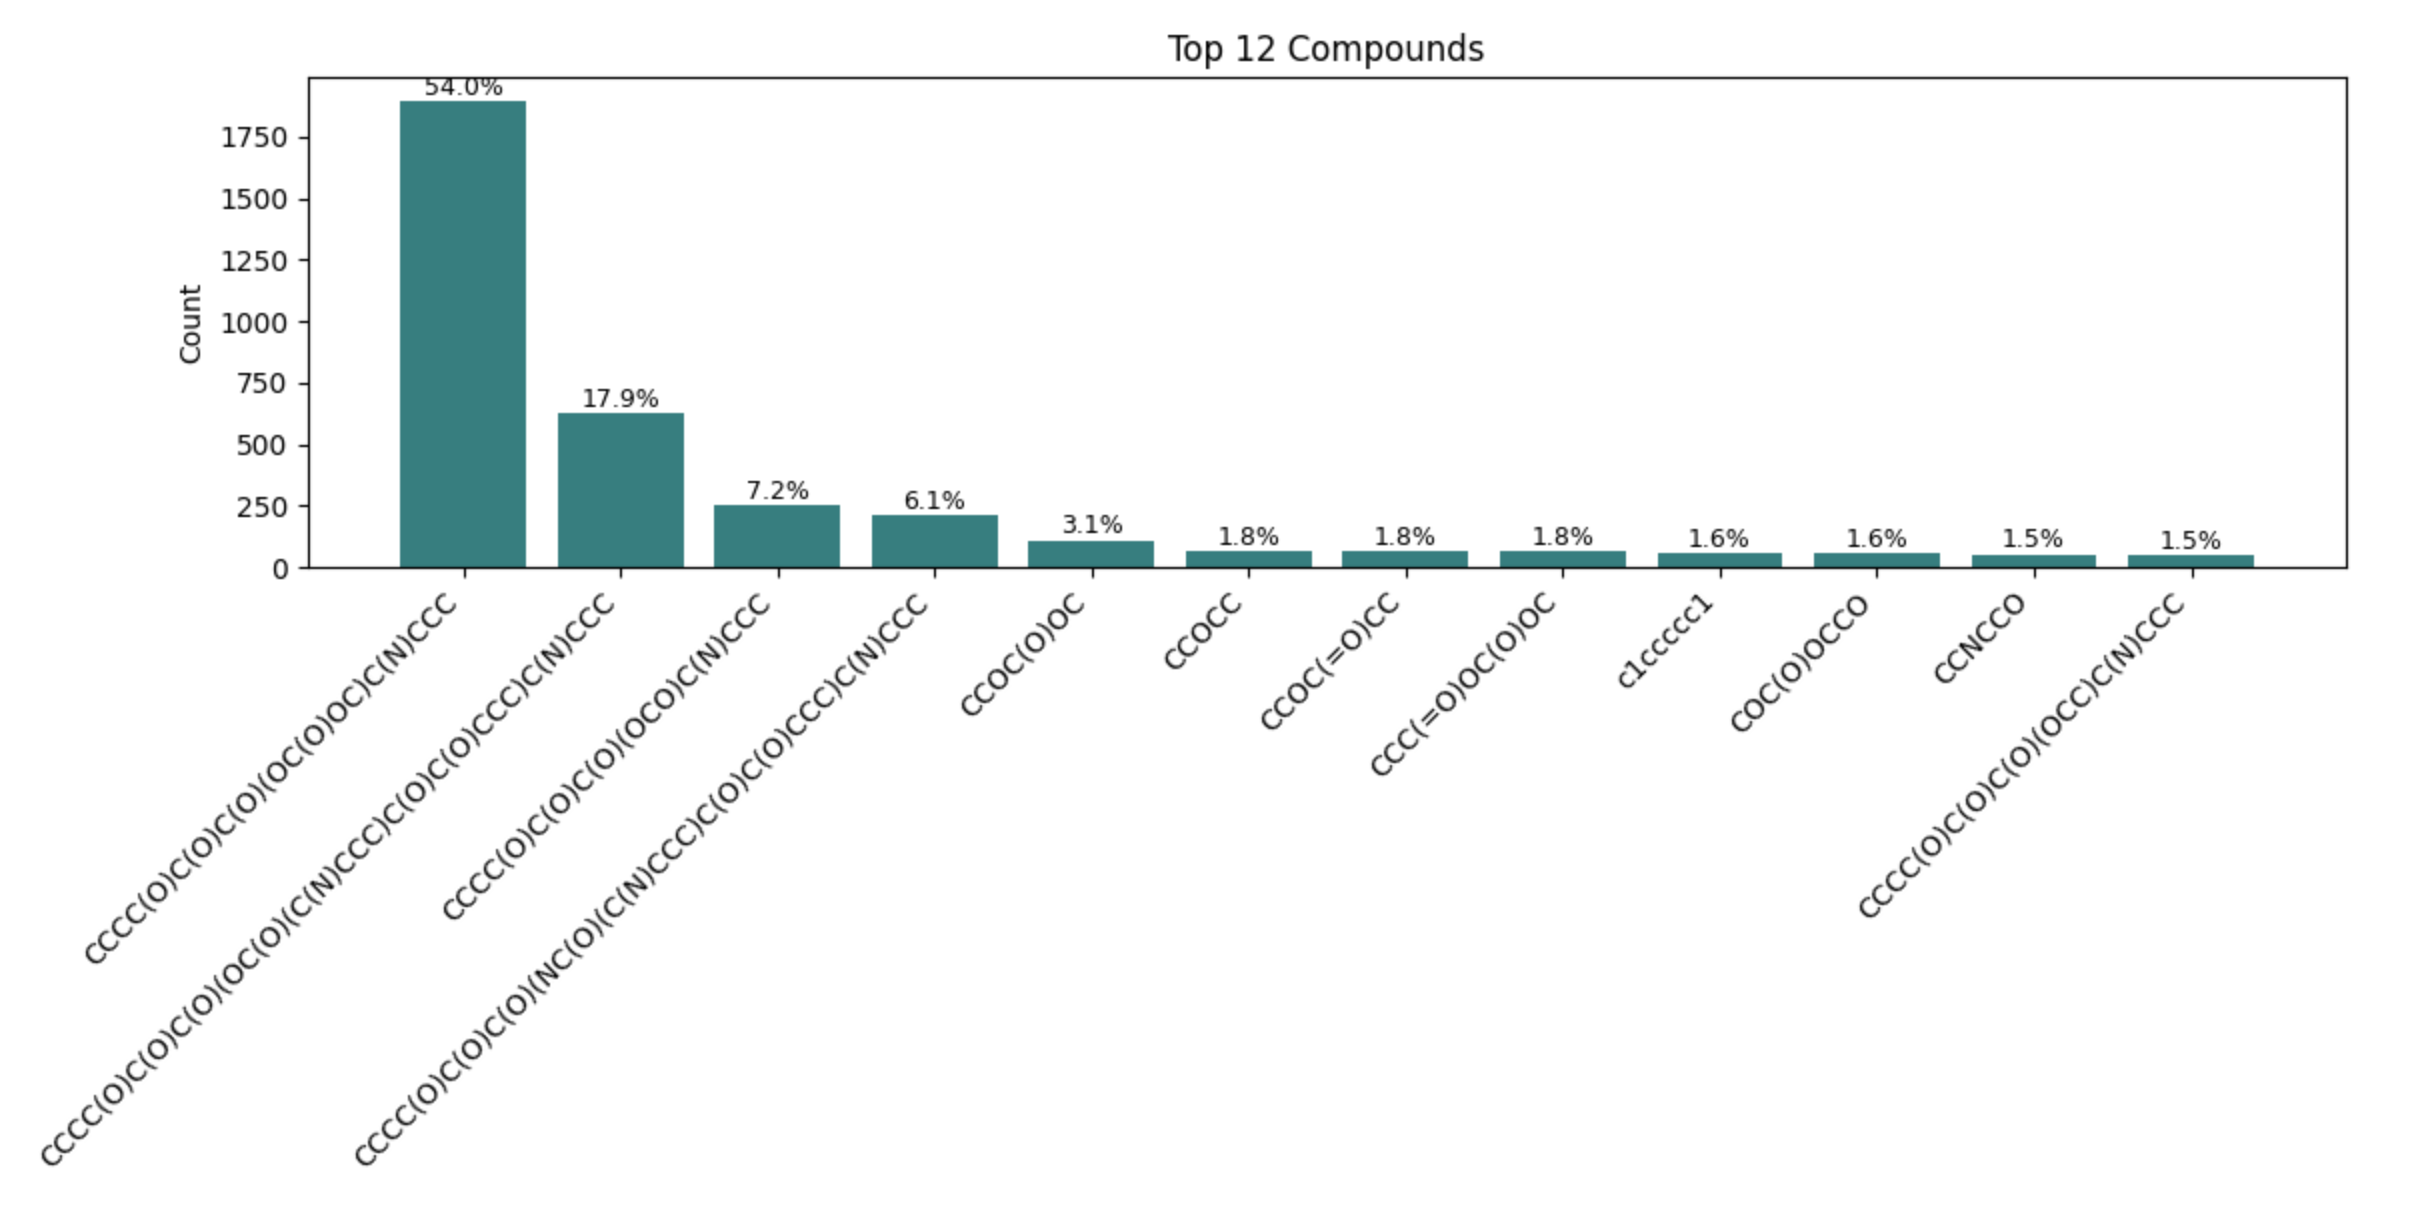
\includegraphics[width=\fulllength]{SDA-chem-hist.png}
\end{adjustwidth}
\caption{Histogram of the twelve most frequent compounds at generation 1000, expressed as counts and percentages. One compound accounts for $\sim$54\% of the population, with the next runner-up at $\sim$18\%.}
\label{fig:chem-compound-hist}
\end{figure}

Figure~\ref{fig:chem-compound-hist} shows the distribution of the twelve most abundant compounds in generation 1000. A single ester-like motif (CCCC(O)C(O)C(O)(OC(O)OC)C(N)CCC) dominates more than half of the population ($\sim$54\%), while the second most frequent compound---a recursive oligomer in which the polyol core is extended by an additional C(N)CCC branch---accounts for 18\%. The third and fourth most frequent motifs (at 7\% and 6\%, respectively) are close structural relatives: one retains the O–C(=O)–O ester fragment in a simpler form, while the other incorporates an amide-like NC(O) substitution into the same polyol backbone. Together, these four scaffolds account for over 85\% of the entire pool.

From a GA perspective, this concentration illustrates how roulette-wheel selection emerges naturally from persistence: once a motif survives longer, it contributes disproportionately to the parent pool and thus amplifies its frequency. From a chemical perspective, the winners all share the same polyol–amine backbone, differing only in whether the substituent is ester-like, recursive, or amide-like. In other words, the system converges on a GA schema (the hydroxylated carbon scaffold with an appended amine) and explores variations within that schema, selecting for those with the greatest stability. The dominance of these few compounds therefore reflects both the GA principle of schema preservation and the chemical principle that stable substituents accumulate over evolutionary time.

\begin{figure}[H]
    \begin{adjustwidth}{-\extralength}{0cm}
    \centering
    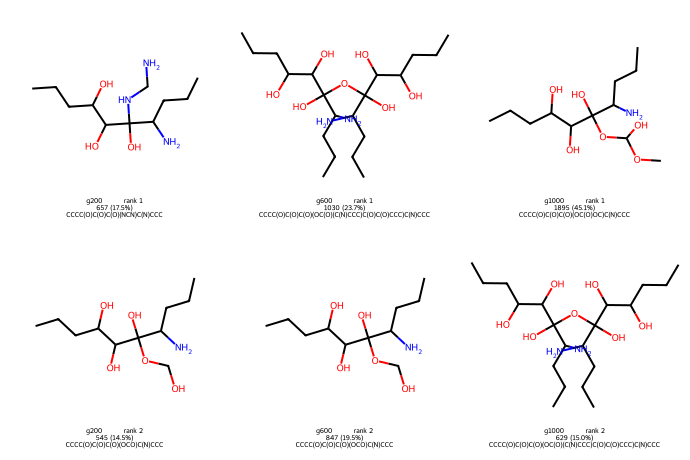
\includegraphics[width=1\textwidth]{SDA-chem-top-evo.png}
    \end{adjustwidth}
    \caption{Evolution of the two top motifs across 200, 600, and 1000 generations. Early competition between aminomethylamino–substituted and ester-like variants gives way to long-term fixation of a single stable scaffold.}
    \label{fig:chem-top-evo}
\end{figure}

Figure~\ref{fig:chem-top-evo} traces the trajectories of the two dominant scaffolds.  
In generation 200, the population is divided between an aminomethylamino–substituted polyol (–NH–CH$_2$–NH$_2$; 17.5\%) and a related ester-like variant (14.5\%), both sharing a hydroxylated backbone with an appended amine chain.

By generation 600, a recursive oligomer elaborating the aminomethylamino–substituted branch expands to 23.7\%, while the ester-like motif remains at 19. 5\%. This phase reflects SDA’s tendency to preserve a common schema while generating more complex derivatives.  

By generation 1000, the simpler ester-like scaffold dominates nearly half of the pool (45. 1\%), while the recursive oligomer decreases to 15. 0\%. The trajectory illustrates schema competition: Multiple variants emerge from a shared template, but persistence imbalances ultimately favor the scaffold that best balances stability and generativity. Chemically, this shows how modest substituents (ester-like O–C(=O)–O groups) can outperform bulkier elaborations, driving convergence on motifs that are robust and reproductively generative.


\begin{figure}[H]
\centering
\subfloat[\centering Entropy dynamics]{
    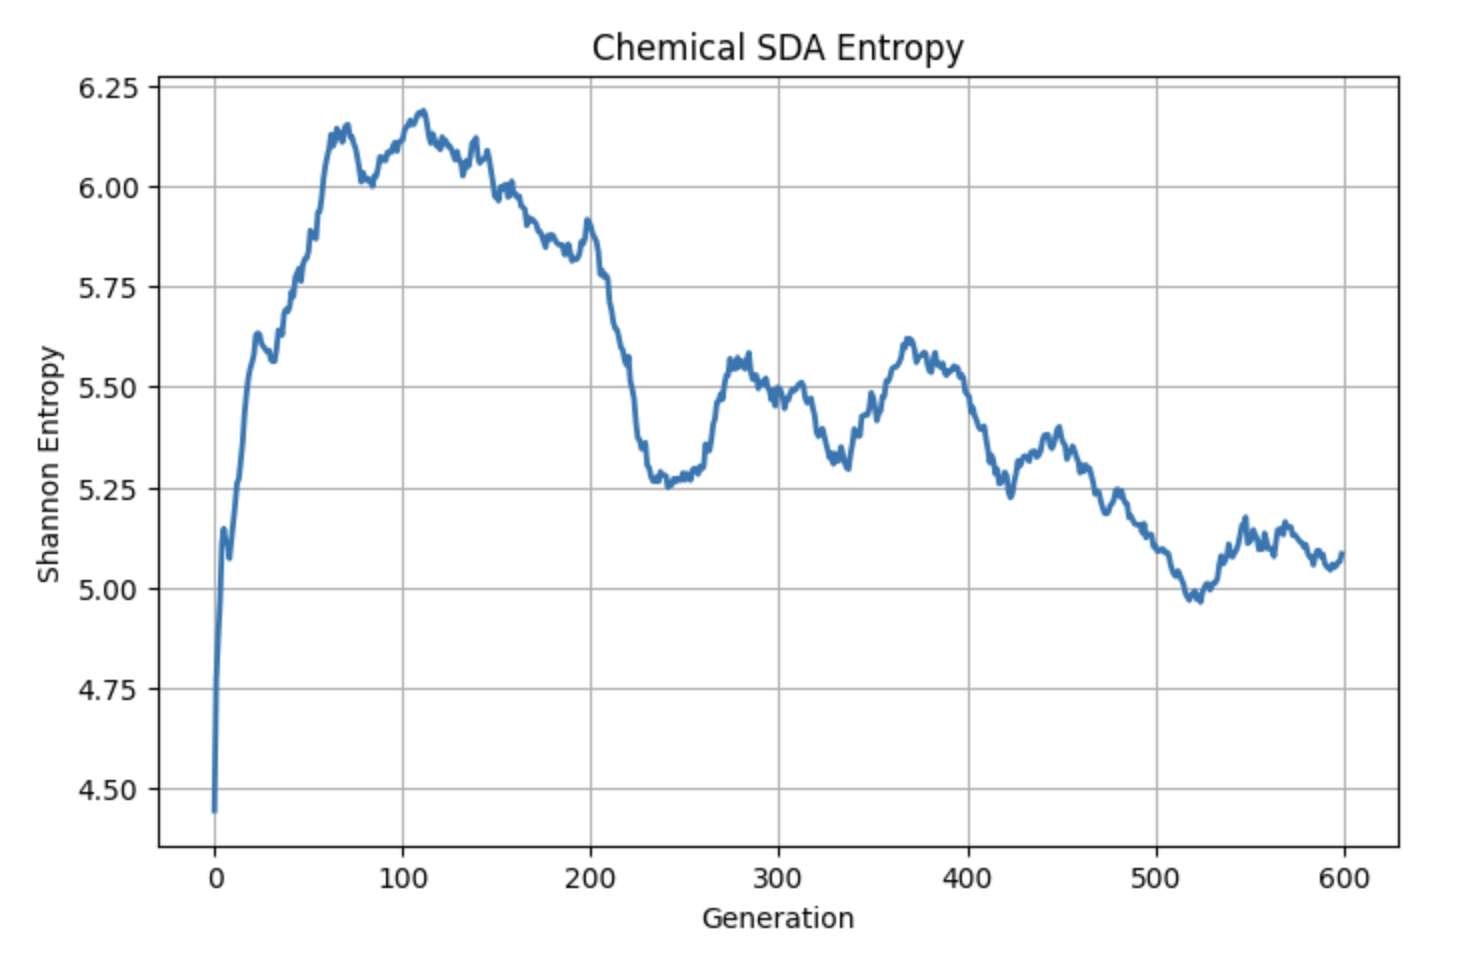
\includegraphics[width=0.45\textwidth]{SDA-chem-entropy.png}
    \label{fig:chem-entropy}
}
\hfill
\subfloat[\centering Diversity dynamics]{
    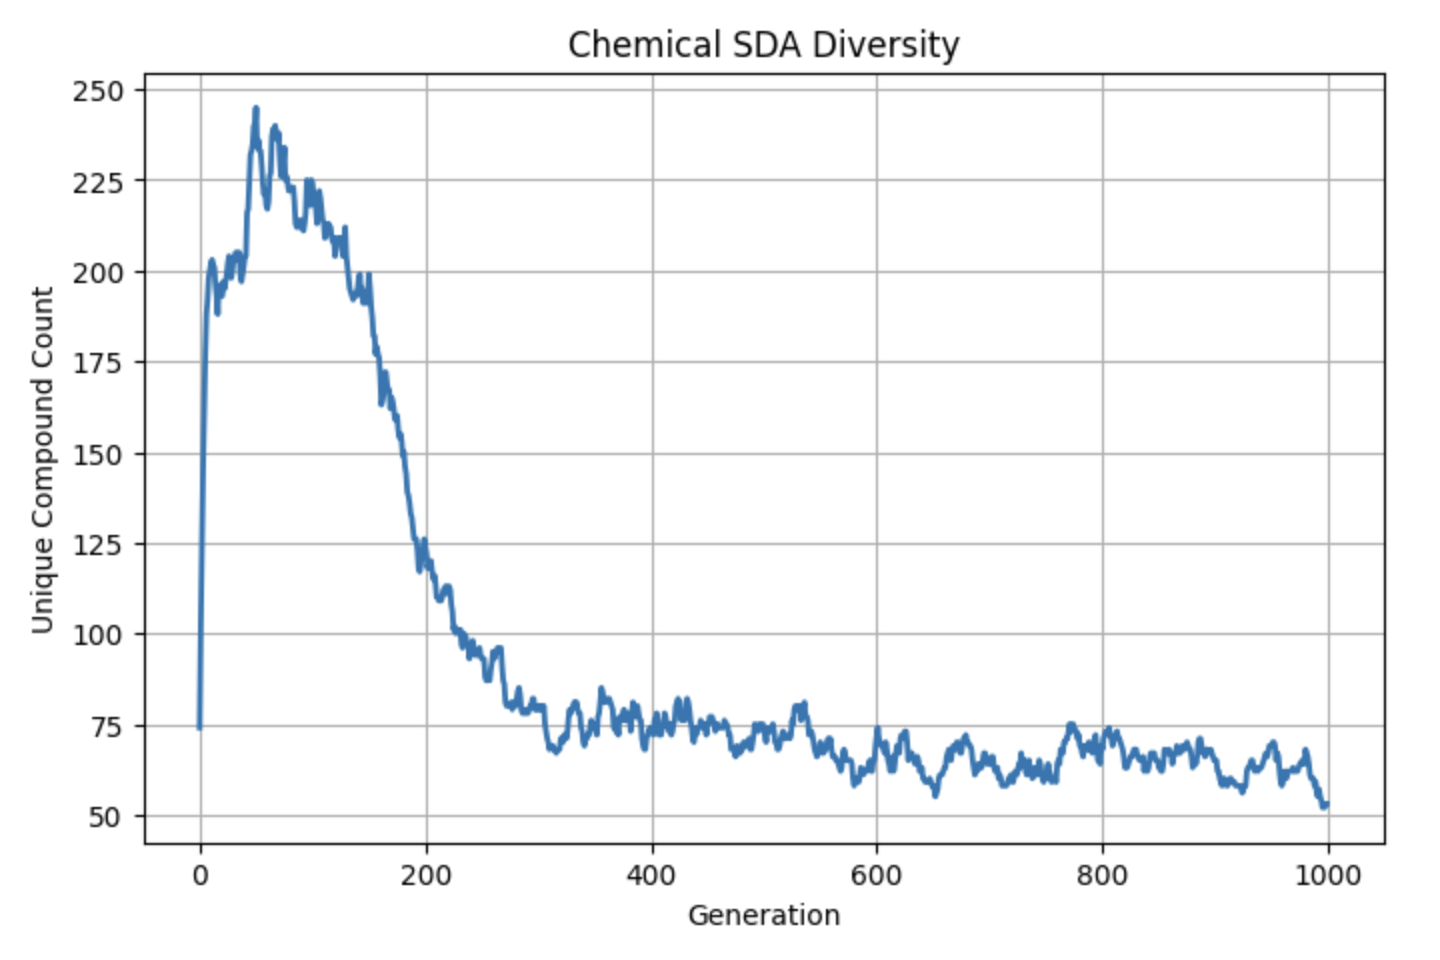
\includegraphics[width=0.45\textwidth]{SDA-chem-diversity.png}
    \label{fig:chem-diversity}
}
\caption{System-level traces of chemical SDA. (\textbf{a}) Shannon entropy rises sharply as new compounds appear, then declines steadily as dominant motifs consolidate. (\textbf{b}) Unique compound diversity follows a parallel trajectory, peaking at over 200 species before collapsing to $\sim$50 by the end of the run.}
\label{fig:chem-entropy-diversity}
\end{figure}

The entropy and diversity dynamics, shown in Figure~\ref{fig:chem-entropy-diversity}, both trace the consolidation of the system. During the first 100-200 generations, the entropy increases and the diversity expands to more than 200 distinct compounds as exploration dominates. Thereafter, both measures decline in parallel: entropy falls steadily, while diversity collapses to about 50 species by generation 1000, with the vast majority of the population concentrated in just two scaffolds. Together, these trends show how stability-driven persistence prunes the search space, channeling the system toward a narrowed set of long-lived motifs.


\begin{figure}[H]
\centering
\subfloat[\centering Novelty over time]{
    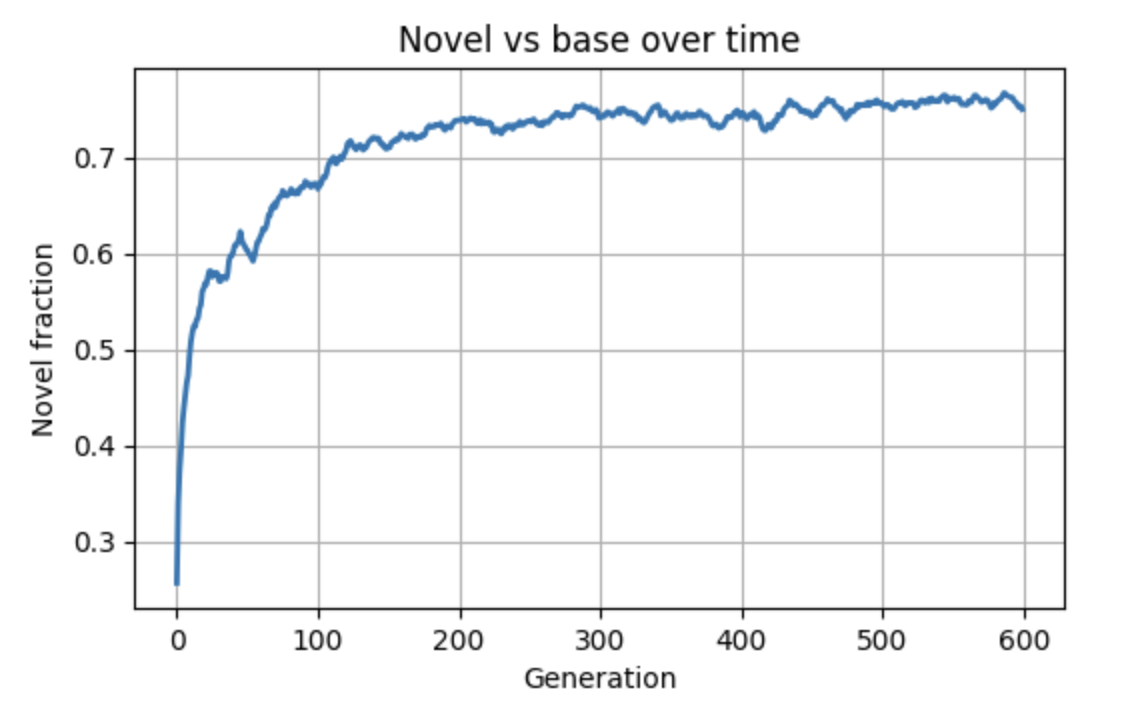
\includegraphics[width=0.45\textwidth]{SDA-chem-novel.png}
    \label{fig:chem-novel}
}
\hfill
\subfloat[\centering Rank--abundance distribution]{
    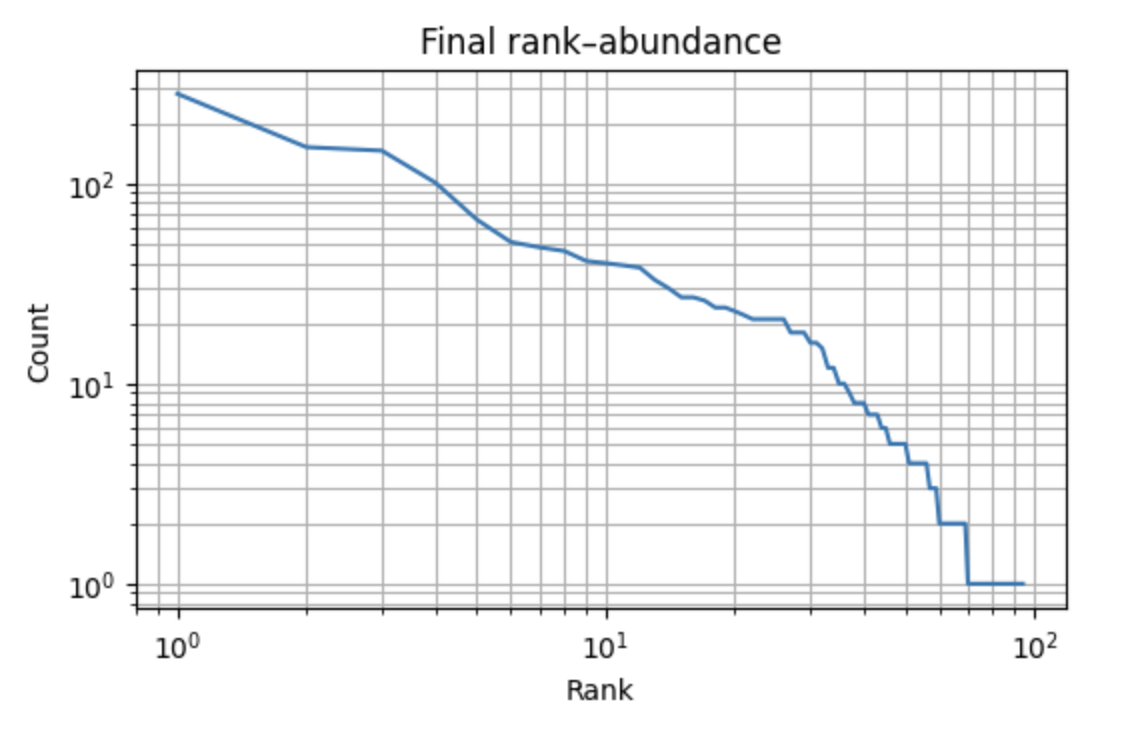
\includegraphics[width=0.45\textwidth]{SDA-chem-rank.png}
    \label{fig:chem-rank}
}
\caption{Novelty and abundance structure in chemical SDA. (\textbf{a}) Fraction of novel compounds (not present in the initial fragment pool) over time. Novelty rapidly overtakes the base pool and stabilizes above 80\%. (\textbf{b}) Rank--abundance distribution at generation 1000 (log--log scale), showing a heavy-tailed form where a few motifs dominate while many persist at low frequency.}
\label{fig:chem-novel-rank}
\end{figure}

The structure of the novelty and abundance is summarized in Figure~\ref{fig:chem-novel-rank}. The fraction of novel compounds increases dramatically and exceeds 80\% in generation 200, remaining stable thereafter. This shows that evolutionary dynamics are driven by new recombinations rather than simple recycling of the initial pool, making novelty a sustained rather than transient feature. At the same time, the final population adopts a heavy-tailed rank--abundance distribution: a small number of motifs dominate by orders of magnitude, while a long tail of rare compounds persists at low frequency. Together, these results demonstrate that SDA dynamics not only sustain open-ended exploration but also generate structured, law-like abundance patterns closely analogous to those observed in ecological systems.


\subsection{Interpretation}

These results show that chemical SDA mirrors the dynamics of a natural GA. Population skew arises spontaneously from persistence imbalances: compounds that survive longer contribute disproportionately to the parent pool, creating effective roulette-wheel selection without an explicit fitness function. This mechanism is evident in the histogram and motif trajectories (Figures~\ref{fig:chem-compound-hist}, \ref{fig:chem-top-evo}), which show oligopolistic dominance and scaffold-level competition.  

System-level traces (Figures~\ref{fig:chem-entropy}--\ref{fig:chem-novel}) explain how this outcome emerges: entropy and diversity expand initially but collapse as selection narrows the space, while novelty remains high as new motifs continually replace base fragments. The final rank–abundance distribution (Figure~\ref{fig:chem-rank}) underscores that these dynamics are not idiosyncratic but follow statistical patterns seen across complex adaptive systems.  

Even with a simplified stability function, the most abundant compounds exhibit chemically plausible motifs such as polyols, esters, and amine substituents. Their persistence is not arbitrary, but arises from their ability to withstand turnover in the generative environment. These findings support the SDA hypothesis that stability alone, when coupled with recombination and mutation, can drive both the generation of novelty and the convergence on structured, high-complexity attractors, plausibly capturing the dynamics that underlie prebiotic chemical evolution.  


\subsection{Equilibrium Models versus Selection-Driven Evolution}

It is useful to contrast these results with equilibrium-based analyses such as those presented by Mass–Action Kinetics (MAK) models
\cite{fogler1999chemical,TuranyiTomlin2014}. In order to render the governing equations linear and analytically tractable, equilibrium models typically assume constant reaction rates and well-mixed dynamics. This assumption ensures mathematical stability, but also suppresses the very features that drive open-ended evolution. With constant rates, all species are treated as equivalent participants in a Markovian flow, and the long-term behavior is dominated by equilibrium concentrations determined by stoichiometry rather than by persistence differentials. In such a setting, once equilibrium is reached, no further directional change occurs.

In contrast, the SDA framework does not impose constant rates or equilibrium conditions. Instead, the effective lifetime of each compound depends on its stability, so turnover is inherently nonuniform. This creates persistence imbalances: more stable motifs accumulate, while less stable ones vanish, skewing the population distribution and weighting the parent-selection process. As demonstrated in the simulations above, this skew is precisely what produces evolutionary search dynamics. Entropy and diversity expand initially but then collapse as a few stable motifs dominate, novelty is continually generated through recombination, and population abundance assumes a heavy-tailed form reminiscent of ecological communities. None of these features emerges from an equilibrium analysis with constant rates, because such models erase the role of selection in shaping the trajectory of the system.

In short, equilibrium approaches such as MAK characterize the static end state of a reaction network, whereas SDA captures its inherently evolutionary nature. What appears in equilibrium theory as a steady-state distribution is, in the SDA view, the transient outcome of continual competition, turnover, and selection. This distinction highlights why stability-driven selection is indispensable for understanding how chemical systems can move beyond equilibrium chemistry toward open-ended evolution.


\subsection{Contrast to Supervised Learning and Genetic Programming}  

It is also important to distinguish chemical SDA from supervised learning and from conventional genetic algorithms or genetic programming systems. In supervised machine learning, the search is explicitly directed toward minimizing an externally defined loss function. In many GA and GP implementations, the search is likewise guided by a user-specified fitness function that encodes the target solution. In contrast, the chemical SDA-GA has no external objective: it is not guided toward reproducing a particular pattern or solving a predefined optimization problem. Instead, its dynamics are similar to reinforcement learning in an emergent environment, where the only 'reward' signal is persistence. Molecules that survive longer contribute more offspring, and the evolving environment itself continuously reshapes which motifs are viable. The result is an open-ended evolutionary process in which populations adapt toward more stable, better-fitting solutions, not because such solutions were prespecified, but because they emerge as the natural consequence of persistence imbalances in a stochastic chemical landscape.

\subsection{Emergence of a Natural Genetic Algorithm}

\begin{figure}[H]
    \centering
    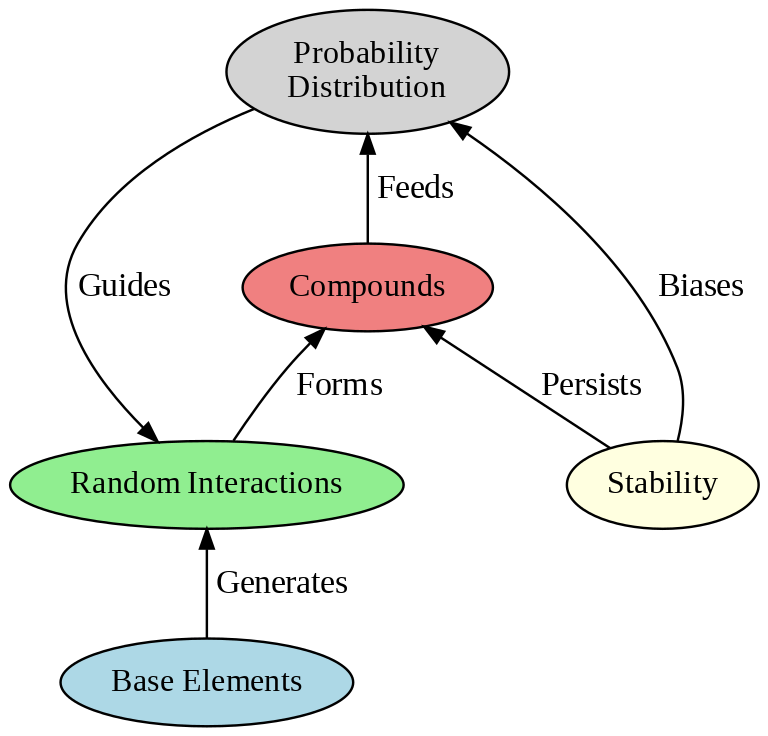
\includegraphics[width=0.6\textwidth]{SDA-top-down.png}
    \caption{Feedback structure underlying chemical SDA dynamics. Base elements interact randomly to form compounds. Compounds that persist contribute more to the population, biasing the probability distribution. This distribution in turn guides future interactions, closing a feedback loop. The result is emergent roulette-wheel selection.}
    \label{fig:top-down}
\end{figure}

The feedback structure shown in Figure~\ref{fig:top-down} provides a mechanistic explanation for how the GA-like search spontaneously emerges in chemical SDA. In conventional genetic algorithms, roulette-wheel selection is imposed externally: the algorithm samples parents in proportion to a programmer-defined fitness function. In SDA, no such programmer is required. Instead, stability imbalances ensure that some compounds persist longer than others. Persistence in turn biases the probability distribution over the population, which then guides future interactions. 

This feedback loop closes the causal chain: the compounds shape the distribution, the distribution shapes sampling, and sampling determines which compounds are likely to interact. In effect, the selection pressure is not imposed top-down, but emerges bottom-up from the persistence differences within the population. The result is indistinguishable from roulette-wheel selection, yet it arises naturally from the dynamics of the system.

This perspective also clarifies the often misused notion of top-down causation \cite{noble_dance}. There is no need to posit a mystical programmer or abstract force directing the search. What appears as a top-down influence of the probability distribution on individual elements is mechanistically explained by the accumulation of persistence imbalances at the population level. Stability alone suffices to generate the feedback necessary for open-ended, GA-like evolution.


\section{Discussion and Implications}

\subsection{Open-Endedness and Computation}
SDA can be viewed as a Markov process on an effectively unbounded state space. 
Unlike equilibrium models that converge to fixed points, SDA dynamics continually expands the frontier of accessible motifs through recombination and mutation. 
Kauffman's 'adjacent possible' \cite{kauffman2019adjacent} becomes quantifiable: each generation samples a probabilistic frontier rather than looking for a target.  

This perspective links SDA to computation. Genetic programming showed that variation and selection can evolve nontrivial algorithms; SDA suggests that matter itself may evolve universal computation. Where Lloyd \cite{{lloyd2006programming}} portrays the universe as computing via bottom–up bit flips, SDA represents a self-modifying computation driven by feedback between persistence landscapes and assembly dynamics: generative rather than simulative.

\subsection{The Evolutionary Ladder Hypothesis}  

\begin{figure}[H]
\centering
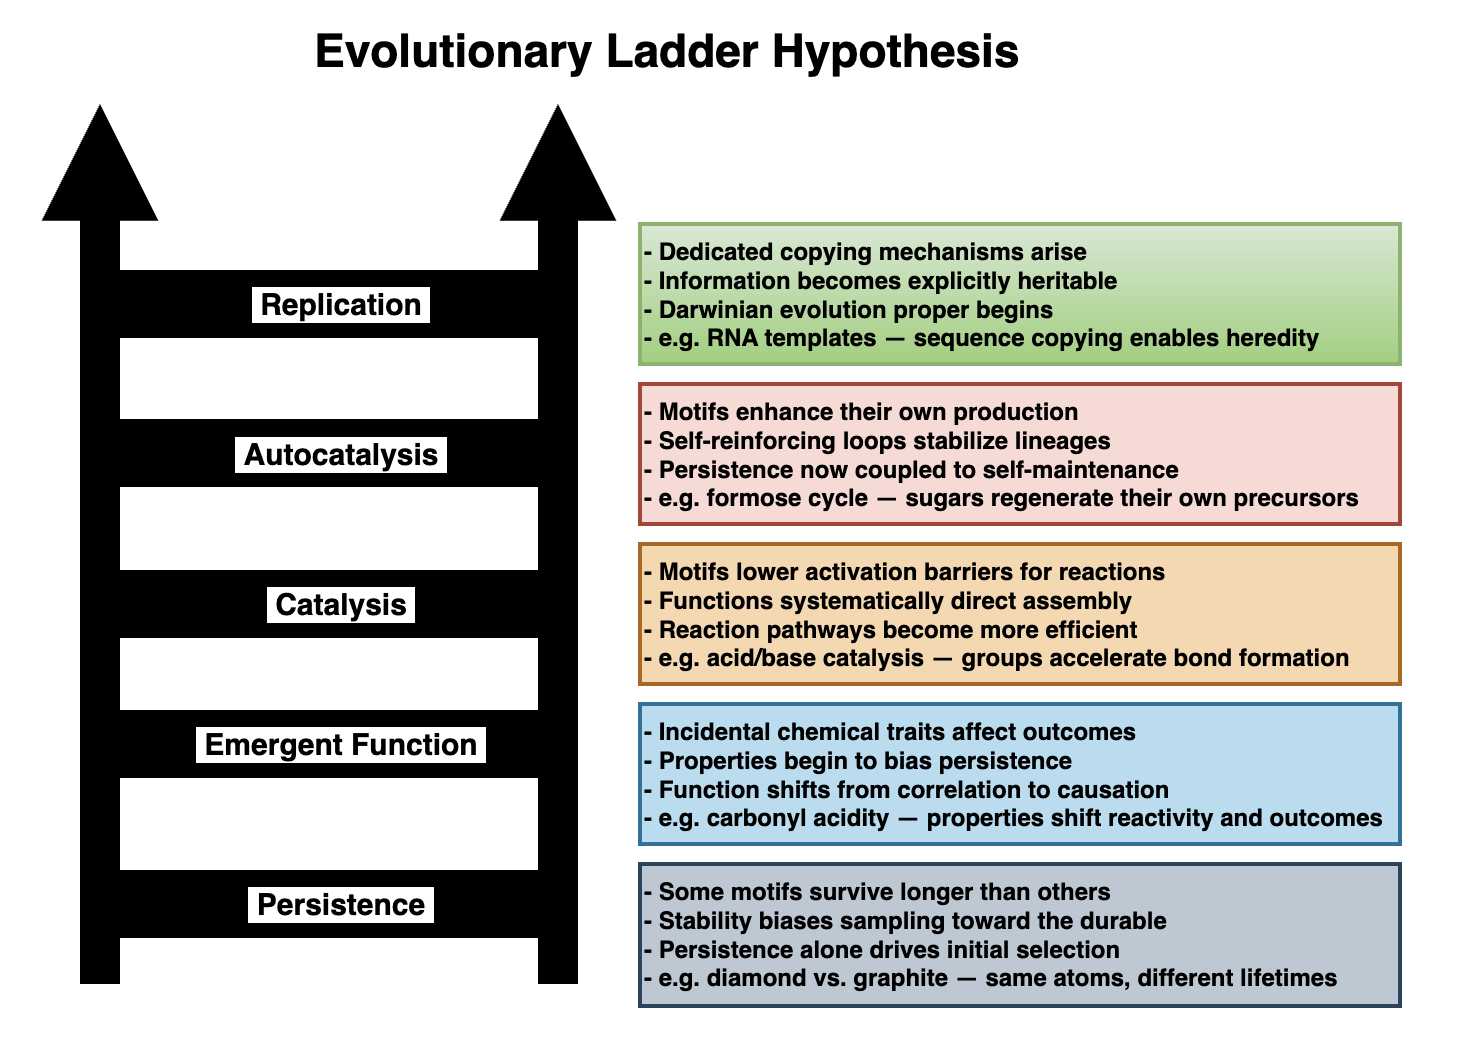
\includegraphics[width=\textwidth]{SDA-ladder.png}
\caption{\textbf{SDA Evolutionary Ladder.} A stepwise progression from persistence-only dynamics to Darwinian replication. 
Rungs (bottom$\rightarrow$top): \emph{Persistence}—some motifs are longer-lived, biasing sampling; 
\emph{Emergent Function}—incidental chemical properties begin to bias persistence and can become causal; 
\emph{Catalysis}—functional motifs systematically lower barriers and direct assembly; 
\emph{Autocatalysis}—motifs enhance their own production, forming self-reinforcing loops; 
\emph{Replication}—sequence-specific copying makes information explicitly heritable. 
The boxes at right give concise examples for each rung (e.g., diamond vs.\ graphite; carbonyl acidity; acid/base catalysis; the formose cycle; RNA templating). 
Colors encode increasing organizational complexity.}
\label{fig:sda-ladder}
\end{figure}

Figure~\ref{fig:sda-ladder} illustrates the evolutionary ladder hypothesis, a proposed continuum linking chemistry to biology. At the base lies \emph{persistence}: Some motifs simply last longer than others. Diamonds outlast graphite under pressure, and stable scaffolds remain in circulation while unstable ones vanish. In this phase, persistence alone biases sampling, creating the first form of selection without function.  

The next rung, \emph{emergent function}, arises when incidental chemical traits begin to influence persistence. For example, a carbonyl motif that mutates into a carboxylic acid changes acidity, altering how it interacts with the environment. In SDA terms, this is a single mutation, but chemically it shifts reactivity, allowing the motif to persist in contexts where neutrality would not. At this stage, properties are still largely correlated with persistence, but they begin to bias outcomes systematically.  

A concrete example illustrates the transition from correlation to causation. Consider a carbonyl mutating into a carboxylic acid. The acid group can protonate bases and lower activation barriers, thereby catalyzing an unrelated condensation reaction that produces a more persistent ester or amide motif. In SDA terms, the first motif’s persistence is no longer merely correlated with stability: its functional effect causally increases the survival and reproduction of another motif. The second motif then increases in frequency not only due to its intrinsic stability, but because the acid \emph{phenotypic function} enabled its production. Function thus feeds directly into the feedback loop of persistence, transforming passive traits into causal drivers of selection.  

This transition naturally leads to \emph{catalysis}, where the motifs systematically lower the activation barriers, channeling reaction pathways toward more efficient outcomes. Once catalysis is established, some motifs go further, entering \emph{autocatalysis}. In this rung, motifs not only stabilize others, but reinforce their own production. The formose sugar cycle, for example, regenerates its own intermediates, creating a self-reinforcing lineage. Persistence is now coupled to self-maintenance.  

Finally, \emph{replication} \cite{england2013statphys} emerges when the copying mechanisms become explicit and sequence-specific. At this rung, information is no longer implicit in persistence alone, but is encoded in heritable structures such as RNA templates. Darwinian evolution proper begins only here, when variation, inheritance, and selection operate together.  

Seen as a continuum, replication is therefore not the foundation of evolution but one rung in a broader ladder that begins with persistence. Our simulations capture the earliest stages, showing that persistence imbalances alone can launch evolutionary trajectories, with phenotypic functions serving as the bridge from chemistry to biology.


\subsection{Echoes in Biology}

Patterns reminiscent of persistence-driven selection can be found at multiple levels of biology.  
At the genomic scale, \textit{selfish elements} such as transposons may persist in lineages largely because they survive long enough to bias inheritance, while \textit{codon usage bias} has been associated with stability in translational dynamics \cite{hershberg2008codon}. 
At the organismal scale, traits that extend lifespan can influence population outcomes beyond immediate reproduction, in ways captured by the covariance structure of Price’s equation \cite{price1970}.  
At the ecological scale, long-lived keystone species stabilize communities and bias viable interactions \cite{mills1993keystone}.  

These examples do not imply identical mechanisms, but they highlight recurring feedback cycles in which stability extends persistence, persistence biases sampling, and biased sampling influences outcomes.  
The parallels with our chemical simulations suggest that persistence-based dynamics may be a broadly relevant theme, potentially linking processes across chemistry, biology, and ecology.


\subsection{Hardware–Software Analogy in Origins Models}

Origins-of-life models are sometimes framed in terms of a hardware/software analogy, 
with chemistry providing the hardware \cite{fontana1991algorithmic, cronin2024chemputation} and genetic sequences providing the software. This metaphor underlies the RNA world hypothesis \cite{gesteland2006rna}, where RNA is cast as both a catalyst and a code. 
Yet the analogy leaves open how integrated systems such as the ribosome–genome complex could have emerged \cite{maynardsmith1999origins}. 

SDA/GA reframes the issue by applying persistence to the system as a whole.  
In this view, both the “hardware” (molecular structures with finite lifetimes) 
and the “software” (patterns that bias future assemblies) contribute to persistence 
and are therefore subject to the same selection-like dynamics.  
As outlined in the evolutionary ladder hypothesis (Fig.~\ref{fig:sda-ladder}), 
this allows optimization to act jointly on structural stability and informational function.  
The hardware/software distinction thus remains a useful analogy, but SDA/GA suggests 
that evolutionary improvement does not require a leap between layers: stability-driven 
feedback can couple physical and informational roles within a single framework.


\subsection{Genotype–Phenotype Integration and the Role of Persistence}

The genotype-phenotype distinction is generally taken as axiomatic, but its origins are unclear.  
In SDA/GA, before true replication arises, persistence alone can play both roles:
stable motifs are physical entities that endure (a phenotypic trait) and their persistence biases sampling
as if they were templates (a genotypic role).  

This perspective helps to soften the problem of 'irreducible complexity'.  
Partial motifs need not be fully functional; if they are stable enough, they remain in circulation and
can scaffold the emergence of more elaborate functions.  
As catalytic or structural effects appear, they feed back to increase persistence, shifting the system
upward along the evolutionary ladder (Fig.~\ref{fig:sda-ladder}).  
In this framing, Darwinian replication is not a sharp discontinuity but a rung that builds upon persistence-driven dynamics already in place.


\subsection{Why Uneven Stability Landscapes Are Generic}

Could a universe exhibit uniform persistence across all motifs? Such a
perfectly balanced landscape is combinatorially improbable and thermodynamically uninteresting: There is only one maximum-entropy configuration, whereas there are vastly many uneven ones. Physical constraints
such as valence and geometry further restrict the assembly space, channeling
viability into structured regions. As a result, SDA-like dynamics arise
generically, since stable motifs almost always exist and bias population
distributions by default.


\subsection{Persistence as Open-Ended Optimization}
Because SDA is equivalent to a GA, it inherits the universality of GAs as search procedures. 
The difference is that classical GAs optimize an explicit fitness function, while SDAs optimize nothing external. 
Persistence itself is the criterion: structures that last longer are sampled more often, biasing the search toward longevity. This makes SDA an open-ended optimization process: not directed toward a solution but toward enduring structure. 
The result is a systematic accumulation of order and information without teleology.  

\subsection{Fine-Tuning as an Emergent Illusion}

From the SDA perspective, appeals to fine-tuning for complexity and life
\cite{rees2000six, davies2006goldilocks} are unnecessary. Persistence
imbalances are generic, and their amplification produces structured, evolving
populations. The order that emerges in any SDA universe is necessarily
shaped by its particular stability landscape and therefore always appears
fine-tuned, even though it arises as a natural consequence of persistence in
a stochastic system.


\section{Conclusions}

This work develops \textit{Stability-Driven Assembly} (SDA) as a mechanism by which selection can emerge without explicit fitness functions or replicators. The principle is straightforward: persistence imbalances skew the population, and that skew feeds back into sampling so that longer-lived motifs are chosen more often. The loop \emph{create $\rightarrow$ persist $\rightarrow$ sample} thereby implements the equivalent of roulette–wheel selection—a natural genetic algorithm (SDA/GA) in which fitness is supplied by the environment rather than imposed by a programmer.  

Chemical simulations illustrate these dynamics: populations converge toward dominance by a few scaffolds, entropy and diversity first expand and then contract, and rank–abundance curves acquire heavy tails with a handful of dominant motifs and many rare ones. These are hallmarks of selection acting on a generative process, where novelty is continually introduced but only persistent structures accumulate.  

This perspective contrasts with equilibrium approaches (e.g., constant-rate models in the spirit of MAK), which suppress such feedback by construction. In SDA/GA, effective rates are heterogeneous because stability differs between motifs, making the ``steady state’’ itself an evolving distribution.  

The present formulation remains simplified, relying on heuristic stability functions, abstracted operators, well-mixed dynamics, and the omission of solvent or kinetic detail. Future work should extend these models with multi-run statistics, richer $S(p)$ grounded in thermodynamics and kinetics, additional reaction classes (acid–base cycles, isomerization, polymerization), and experimental tests in open, driven reactors where persistence can be directly measured.  

SDA/GA reframes information not as a pre-existing substance but as an emergent 
property of population dynamics. Regularities accumulate because persistence 
biases which motifs endure and recombine, so that information itself evolves 
through biased exploration. From a population perspective, this process is 
indistinguishable from evolution: order and information emerge as stable 
motifs persist longer, recur more often, and proliferate within the population 
through persistence-driven selection, pointing to a common principle linking 
chemistry, computation, and biology.



\section{Simulation Code}

All Python code and simulation results are openly available at:
\url{https://github.com/danadler-dev/MDPI-Life-Article}. 
The repository README includes a link to an interactive Google Colab notebook with the complete code and outputs corresponding to the figures and experiments presented in this paper.

\begin{adjustwidth}{-\extralength}{0cm}
%\printendnotes[custom] % Un-comment to print a list of endnotes

\reftitle{References}



% Please provide either the correct journal abbreviation (e.g. according to the “List of Title Word Abbreviations” http://www.issn.org/services/online-services/access-to-the-ltwa/) or the full name of the journal.
% Citations and References in Supplementary files are permitted provided that they also appear in the reference list here. 

%=====================================
% References, variant A: external bibliography
%=====================================
% \bibliography{your_external_BibTeX_file}

%=====================================
% References, variant B: internal bibliography
%=====================================

% ACS format
\isAPAandChicago{}{%
\begin{thebibliography}{999}
% Reference 1
\bibitem{ruizmirazo2014}
Ruiz-Mirazo, K.; Briones, C.; de la Escosura, A. 
Prebiotic Systems Chemistry: New Perspectives for the Origins of Life. 
\textit{Chemical Reviews} \textbf{2014}, 114 (1), 285–366. doi:10.1021/cr2004844.

% Reference 2
\bibitem{nghe2015prebiotic}
Nghe, P.; Hordijk, W.; Kauffman, S.A.; Walker, S.I.; Schmidt, F.J.; Kemble, H.; Yeates, J.A.; Lehman, N. \textit{Prebiotic network evolution: Six key parameters.} Molecular BioSystems \textbf{2015}, \textit{11}, 3206–3217.

% Reference 3
\bibitem{kauffman1993origins}
Kauffman, S.A. 
\textit{The Origins of Order: Self-Organization and Selection in Evolution}; 
Oxford University Press: New York, NY, USA, 1993.

% Reference 4
\bibitem{hordijk2012autocatalytic}
Hordijk, W.; Steel, M.; Kauffman, S. \textit{The Structure of Autocatalytic Sets: Evolvability, Enablement, and Emergence.} Acta Biotheoretica \textbf{2012}, \textit{60}, 379–392.

% Reference 5
\bibitem{kauffman1986autocatalytic}
Kauffman, S.A. \textit{Autocatalytic sets of proteins.} Journal of Theoretical Biology \textbf{1986}, \textit{119}, 1–24.

% Reference 6
\bibitem{hordijk2011required}
Hordijk, W.; Kauffman, S.A.; Steel, M. \textit{Required levels of catalysis for emergence of autocatalytic sets in models of chemical reaction systems.} International Journal of Molecular Sciences \textbf{2011}, \textit{12}, 3085–3101.

% Reference 7
\bibitem{eigen}
Eigen M. \textit{The Hypercycle: A Principle of Natural Self-Organization.} Springer, 1979.

% Reference 8
\bibitem{fontana1991algorithmic}
Fontana, W. \textit{Algorithmic chemistry.} Artificial Life II \textbf{1991}, \textit{11}, 159–209.

% Reference 9
\bibitem{adami1994}
Adami, C.; Brown, C.T. 
Evolutionary Learning in the 2D Artificial Life System ``Avida.'' 
\textit{arXiv preprint} adap-org/9405003, 1994. Available online: \url{https://arxiv.org/abs/adap-org/9405003}.

% Reference 10
\bibitem{ray1992tierra}
Ray, T.S. \textit{An approach to the synthesis of life}. Artificial Life II \textbf{1991}, 371--408.

% Reference 11
\bibitem{cronin2024chemputation}
Cronin, L.; Pagel, S.; Sharma, A. \textit{The Chemputer and Chemputation: A Universal Chemical Compound Synthesis Machine}. Preprint available on arXiv (August 2024), arXiv:2408.09171.

% Reference 12
\bibitem{segre2000compositional}
Segre, D.; Ben-Eli, D.; Lancet, D. \textit{Compositional genomes: Prebiotic information transfer in mutually catalytic noncovalent assemblies}. Proc. Natl. Acad. Sci. USA \textbf{2000}, 97, 4112--4117.

% Reference 13
\bibitem{markovitch2012universal}
Markovitch, O.; Lancet, D. \textit{Excess mutual catalysis is required for effective evolvability}. Artif. Life \textbf{2012}, 18, 243--266.

% Reference 14
\bibitem{damer2015coupled}
Damer, B.; Deamer, D. \textit{Coupled phases and combinatorial selection in fluctuating hydrothermal pools: A scenario to guide experimental approaches to the origin of cellular life}. Astrobiology \textbf{2015}, 15, 861--877.

% Reference 15
\bibitem{barabasi1999emergence}
Barabási, A.-L.; Albert, R. \textit{Emergence of Scaling in Random Networks.} Science \textbf{1999}, \textit{286}, 509–512.

% Reference 16
\bibitem{prigogine1977self}
Prigogine, I.; Nicolis, G. \textit{Self-Organization in Non-Equilibrium Systems}; Wiley: New York, NY, USA, 1977.

% Reference 17
\bibitem{england2015dissipative}
England, J.L. \textit{Dissipative Adaptation in Driven Self-Assembly.} Nature Nanotechnology \textbf{2015}, \textit{10}, 919–923.

% Reference 18
\bibitem{nowak2006evolutionary}
Nowak, M.A. \textit{Evolutionary Dynamics: Exploring the Equations of Life}; Belknap Press: Cambridge, MA, USA, 2006.


% Reference 19
\bibitem{wu2012origin}
Wu, M.; Higgs, P.G. \textit{Origin of self-replicating biopolymers: Autocatalytic feedback can trump power law replication.} Journal of Molecular Evolution \textbf{2012}, \textit{74}, 91–102.

% Reference 20
\bibitem{walker2023nature}
Walker, S.I.; Cronin, L.; et al. \textit{Assembly theory explains and quantifies selection and evolution across physical and biological systems.} Nature 2023, 618, 619-628.

% Reference 21
\bibitem{deutsch2013constructor}
Deutsch, D.; Marletto, C. \textit{Constructor theory of information.} Proceedings of the Royal Society A: Mathematical, Physical and Engineering Sciences \textbf{2015}, \textit{471}, 20140540.

% Reference 22
\bibitem{holland1975adaptation}
Holland, J.H. \textit{Adaptation in Natural and Artificial Systems}; University of Michigan Press: Ann Arbor, MI, USA, 1975.

% Reference 23
\bibitem{adler1993marriage}
Adler, D. \textit{Genetic algorithms and simulated annealing: a marriage proposal}. Proceedings of the IEEE International Conference on Neural Networks, San Francisco, CA, USA, 1993; pp. 1759--1764. doi:10.1109/ICNN.1993.298712.

% Reference 24
\bibitem{adler_sda}
Adler, D.
\textit{Stability-Driven Assembly Theory}.
SSRN Preprint, 2025. Available at: \url{https://dx.doi.org/10.2139/ssrn.5203036}. Submitted to \textit{Journal of Theoretical Biology}.

% Reference 25
\bibitem{fogler1999chemical}
Fogler, H.S. \textit{Elements of Chemical Reaction Engineering} (3rd ed.). Prentice Hall, 1999.

% Reference 26
\bibitem{gardiner2009} Gardiner, C. W. (2009). \textit{Stochastic Methods: A Handbook for the Natural and Social Sciences} (4th ed.). Springer.

% Reference 27
\bibitem{mckean1966}
McKean, H.P. 
\textit{A Class of Markov Processes Associated with Nonlinear Parabolic Equations}. 
Proceedings of the National Academy of Sciences \textbf{1966}, 56, 1907–1911. doi:10.1073/pnas.56.6.1907.

% Reference 28
\bibitem{villani2009}
Villani, C. 
\textit{Optimal Transport: Old and New}. Springer, Berlin, 2009. 
(See Chapter 2 for nonlinear Fokker–Planck and McKean–Vlasov formulations.)

% Reference 29
\bibitem{goldberg1989genetic}
Goldberg, D.E. \textit{Genetic Algorithms in Search, Optimization, and Machine Learning}; Addison-Wesley: Boston, MA, USA, 1989.

% Reference 30
\bibitem{koza1992genetic}
Koza, J. R.
\textit{Genetic Programming: On the Programming of Computers by Means of Natural Selection}.
MIT Press, USA, 1992.

% Reference 31
\bibitem{dawkins1986blind}
Dawkins, R. \textit{The Blind Watchmaker}; W.W. Norton: New York, NY, USA, 1986.

% Reference 32
\bibitem{adler2025jazz}
Adler, D. \textit{Active Listening in Jazz}. Available online: \url{https://jazzintro.com}.

% Reference 33
\bibitem{brown2004ga}
Brown, N.; McKay, B.; Gilardoni, F.; Gasteiger, J.
\textit{A graph-based genetic algorithm and its application to the multiobjective
evolution of median molecules.}
J. Chem. Inf. Comput. Sci. 2004, 44, 1079--1087.

% Reference 34
\bibitem{lewis1998gp}
Lewis, R. A.
\textit{Genetic programming as a model for drug design.}
J. Chem. Inf. Comput. Sci. 1998, 38, 651--657.

% Reference 35
\bibitem{jensen2019ga}
Jensen, J. H.
\textit{A graph-based genetic algorithm and generative model/GA hybrid for molecular discovery.}
Chem. Sci. 2019, 10, 3567--3572.

% Reference 36
\bibitem{yoshikawa2018ga}
Yoshikawa, N.; Terayama, K.; Sumita, M.; Homma, T.; Oono, K.; Tsuda, K.
\textit{Population-based de novo molecule generation, using grammatical evolution.}
Chem. Lett. 2018, 47, 1431--1434.

% Reference 37
\bibitem{fink2007gdb11}
Fink, T.; Reymond, J.-L.
\textit{Virtual exploration of the chemical universe up to 11 atoms of C, N, O, F:
Assembly of 26.4 million structures (GDB-11).}
J. Chem. Inf. Model. 2007, 47, 342--353.

% Reference 38
\bibitem{landrum2006rdkit}
Landrum, G. (2006). \textit{RDKit: Open-source cheminformatics}. Available at: \url{http://www.rdkit.org}.

% Reference 39
\bibitem{degen2008art}
Degen, J., Wegscheid-Gerlach, C., Zaliani, A., Rarey, M. (2008).
\textit{On the art of compiling and using ‘drug-like’ chemical fragment spaces}.
\textit{ChemMedChem}, 3(10), 1503–1507. https://doi.org/10.1002/cmdc.200800178

% Reference 40
\bibitem{janet2023bestpractices}
Janet, J. P., Duan, C., Yang, T., Kulik, H. J. (2023).
\textit{Determining best practices for using genetic algorithms in molecular discovery}.
\textit{Journal of Chemical Physics}, 159(9), 091501. https://doi.org/10.1063/5.0158336

% Reference 41
\bibitem{TuranyiTomlin2014}
Turányi, T.; Tomlin, A.S. \textit{Analysis of Kinetic Reaction Mechanisms}; Springer: Berlin, Germany, 2014.

% Reference 42
\bibitem{noble_dance}
Noble, D. 
\textit{Dance to the Tune of Life: Biological Relativity}. 
Cambridge University Press: Cambridge, UK, 2017. 
doi:10.1017/CBO9781316403571.

% Reference 43
\bibitem{kauffman2019adjacent}
Kauffman, S.A. 
\textit{Beyond Borders: The Emergence of the Adjacent Possible}. 
Journal of Theoretical Biology \textbf{2019}, \textit{461}, 109--118. 
doi:10.1016/j.jtbi.2018.10.015.

% Reference 44
\bibitem{lloyd2006programming}
Lloyd, S. \textit{Programming the Universe: A Quantum Computer Scientist Takes on the Cosmos}; Alfred A. Knopf: New York, NY, USA, 2006.

% Reference 45
\bibitem{england2013statphys}
England, J.L. 
\textit{Statistical Physics of Self-Replication.} 
Journal of Chemical Physics 2013, \textit{139}, 121923. 
https://doi.org/10.1063/1.4818538.

% Reference 46
\bibitem{hershberg2008codon}
Hershberg, R.; Petrov, D.A. 
\textit{Selection on codon bias.} 
Annual Review of Genetics \textbf{2008}, \textit{42}, 287--299. 
doi:10.1146/annurev.genet.42.110807.091442.

% Reference 47
\bibitem{mills1993keystone}
Mills, L.S.; Soulé, M.E.; Doak, D.F. 
\textit{The Keystone-Species Concept in Ecology and Conservation.} 
BioScience \textbf{1993}, \textit{43} (4), 219--224. 
doi:10.2307/1312122.

% Reference 48
\bibitem{gesteland2006rna}
Gesteland, R.F.; Cech, T.R.; Atkins, J.F. (Eds.) 
\textit{The RNA World}, 3rd ed.; Cold Spring Harbor Laboratory Press: Cold Spring Harbor, NY, USA, 2006. 

% Reference 49
\bibitem{maynardsmith1999origins}
Maynard Smith, J.; Szathmáry, E. 
\textit{The Origins of Life: From the Birth of Life to the Origin of Language}; 
Oxford University Press: Oxford, UK, 1999.

% Reference 50
\bibitem{price1970}
Price, G.R. \textit{Selection and Covariance.} Nature 1970, 227, 520–521 doi:10.1038/227520a0.

% Reference 51
\bibitem{rees2000six}
Rees, M. \textit{Just Six Numbers: The Deep Forces That Shape the Universe}; Basic Books: New York, NY, USA, 2000.

% Reference 52
\bibitem{davies2006goldilocks}
Davies, P. \textit{The Goldilocks Enigma: Why is the Universe Just Right for Life?}; Allen Lane: London, UK, 2006.

\end{thebibliography}
}



% If authors have biography, please use the format below
%\section*{Short Biography of Authors}
%\bio
%{\raisebox{-0.35cm}{\includegraphics[width=3.5cm,height=5.3cm,clip,keepaspectratio]{Definitions/author1.pdf}}}
%{\textbf{Firstname Lastname} Biography of first author}
%
%\bio
%{\raisebox{-0.35cm}{\includegraphics[width=3.5cm,height=5.3cm,clip,keepaspectratio]{Definitions/author2.jpg}}}
%{\textbf{Firstname Lastname} Biography of second author}

% For the MDPI journals use author-date citation, please follow the formatting guidelines on http://www.mdpi.com/authors/references
% To cite two works by the same author: \citeauthor{ref-journal-1a} (\citeyear{ref-journal-1a}, \citeyear{ref-journal-1b}). This produces: Whittaker (1967, 1975)
% To cite two works by the same author with specific pages: \citeauthor{ref-journal-3a} (\citeyear{ref-journal-3a}, p. 328; \citeyear{ref-journal-3b}, p.475). This produces: Wong (1999, p. 328; 2000, p. 475)

%%%%%%%%%%%%%%%%%%%%%%%%%%%%%%%%%%%%%%%%%%
%% for journal Sci
%\reviewreports{\\
%Reviewer 1 comments and authors’ response\\
%Reviewer 2 comments and authors’ response\\
%Reviewer 3 comments and authors’ response
%}
%%%%%%%%%%%%%%%%%%%%%%%%%%%%%%%%%%%%%%%%%%
\PublishersNote{}
%\isPreprints{} % If the paper is ``preprints'', please uncomment this parenthesis.
\end{document}

